% Options for packages loaded elsewhere
\PassOptionsToPackage{unicode}{hyperref}
\PassOptionsToPackage{hyphens}{url}
%
\documentclass[
  ,man,floatsintext]{apa6}
\usepackage{amsmath,amssymb}
\usepackage{lmodern}
\usepackage{iftex}
\ifPDFTeX
  \usepackage[T1]{fontenc}
  \usepackage[utf8]{inputenc}
  \usepackage{textcomp} % provide euro and other symbols
\else % if luatex or xetex
  \usepackage{unicode-math}
  \defaultfontfeatures{Scale=MatchLowercase}
  \defaultfontfeatures[\rmfamily]{Ligatures=TeX,Scale=1}
\fi
% Use upquote if available, for straight quotes in verbatim environments
\IfFileExists{upquote.sty}{\usepackage{upquote}}{}
\IfFileExists{microtype.sty}{% use microtype if available
  \usepackage[]{microtype}
  \UseMicrotypeSet[protrusion]{basicmath} % disable protrusion for tt fonts
}{}
\makeatletter
\@ifundefined{KOMAClassName}{% if non-KOMA class
  \IfFileExists{parskip.sty}{%
    \usepackage{parskip}
  }{% else
    \setlength{\parindent}{0pt}
    \setlength{\parskip}{6pt plus 2pt minus 1pt}}
}{% if KOMA class
  \KOMAoptions{parskip=half}}
\makeatother
\usepackage{xcolor}
\usepackage{longtable,booktabs,array}
\usepackage{calc} % for calculating minipage widths
% Correct order of tables after \paragraph or \subparagraph
\usepackage{etoolbox}
\makeatletter
\patchcmd\longtable{\par}{\if@noskipsec\mbox{}\fi\par}{}{}
\makeatother
% Allow footnotes in longtable head/foot
\IfFileExists{footnotehyper.sty}{\usepackage{footnotehyper}}{\usepackage{footnote}}
\makesavenoteenv{longtable}
\usepackage{graphicx}
\makeatletter
\def\maxwidth{\ifdim\Gin@nat@width>\linewidth\linewidth\else\Gin@nat@width\fi}
\def\maxheight{\ifdim\Gin@nat@height>\textheight\textheight\else\Gin@nat@height\fi}
\makeatother
% Scale images if necessary, so that they will not overflow the page
% margins by default, and it is still possible to overwrite the defaults
% using explicit options in \includegraphics[width, height, ...]{}
\setkeys{Gin}{width=\maxwidth,height=\maxheight,keepaspectratio}
% Set default figure placement to htbp
\makeatletter
\def\fps@figure{htbp}
\makeatother
\setlength{\emergencystretch}{3em} % prevent overfull lines
\providecommand{\tightlist}{%
  \setlength{\itemsep}{0pt}\setlength{\parskip}{0pt}}
\setcounter{secnumdepth}{-\maxdimen} % remove section numbering
% Make \paragraph and \subparagraph free-standing
\ifx\paragraph\undefined\else
  \let\oldparagraph\paragraph
  \renewcommand{\paragraph}[1]{\oldparagraph{#1}\mbox{}}
\fi
\ifx\subparagraph\undefined\else
  \let\oldsubparagraph\subparagraph
  \renewcommand{\subparagraph}[1]{\oldsubparagraph{#1}\mbox{}}
\fi
\newlength{\cslhangindent}
\setlength{\cslhangindent}{1.5em}
\newlength{\csllabelwidth}
\setlength{\csllabelwidth}{3em}
\newlength{\cslentryspacingunit} % times entry-spacing
\setlength{\cslentryspacingunit}{\parskip}
\newenvironment{CSLReferences}[2] % #1 hanging-ident, #2 entry spacing
 {% don't indent paragraphs
  \setlength{\parindent}{0pt}
  % turn on hanging indent if param 1 is 1
  \ifodd #1
  \let\oldpar\par
  \def\par{\hangindent=\cslhangindent\oldpar}
  \fi
  % set entry spacing
  \setlength{\parskip}{#2\cslentryspacingunit}
 }%
 {}
\usepackage{calc}
\newcommand{\CSLBlock}[1]{#1\hfill\break}
\newcommand{\CSLLeftMargin}[1]{\parbox[t]{\csllabelwidth}{#1}}
\newcommand{\CSLRightInline}[1]{\parbox[t]{\linewidth - \csllabelwidth}{#1}\break}
\newcommand{\CSLIndent}[1]{\hspace{\cslhangindent}#1}
\ifLuaTeX
\usepackage[bidi=basic]{babel}
\else
\usepackage[bidi=default]{babel}
\fi
\babelprovide[main,import]{english}
% get rid of language-specific shorthands (see #6817):
\let\LanguageShortHands\languageshorthands
\def\languageshorthands#1{}
% Manuscript styling
\usepackage{upgreek}
\captionsetup{font=singlespacing,justification=justified}

% Table formatting
\usepackage{longtable}
\usepackage{lscape}
% \usepackage[counterclockwise]{rotating}   % Landscape page setup for large tables
\usepackage{multirow}		% Table styling
\usepackage{tabularx}		% Control Column width
\usepackage[flushleft]{threeparttable}	% Allows for three part tables with a specified notes section
\usepackage{threeparttablex}            % Lets threeparttable work with longtable

% Create new environments so endfloat can handle them
% \newenvironment{ltable}
%   {\begin{landscape}\centering\begin{threeparttable}}
%   {\end{threeparttable}\end{landscape}}
\newenvironment{lltable}{\begin{landscape}\centering\begin{ThreePartTable}}{\end{ThreePartTable}\end{landscape}}

% Enables adjusting longtable caption width to table width
% Solution found at http://golatex.de/longtable-mit-caption-so-breit-wie-die-tabelle-t15767.html
\makeatletter
\newcommand\LastLTentrywidth{1em}
\newlength\longtablewidth
\setlength{\longtablewidth}{1in}
\newcommand{\getlongtablewidth}{\begingroup \ifcsname LT@\roman{LT@tables}\endcsname \global\longtablewidth=0pt \renewcommand{\LT@entry}[2]{\global\advance\longtablewidth by ##2\relax\gdef\LastLTentrywidth{##2}}\@nameuse{LT@\roman{LT@tables}} \fi \endgroup}

% \setlength{\parindent}{0.5in}
% \setlength{\parskip}{0pt plus 0pt minus 0pt}

% Overwrite redefinition of paragraph and subparagraph by the default LaTeX template
% See https://github.com/crsh/papaja/issues/292
\makeatletter
\renewcommand{\paragraph}{\@startsection{paragraph}{4}{\parindent}%
  {0\baselineskip \@plus 0.2ex \@minus 0.2ex}%
  {-1em}%
  {\normalfont\normalsize\bfseries\itshape\typesectitle}}

\renewcommand{\subparagraph}[1]{\@startsection{subparagraph}{5}{1em}%
  {0\baselineskip \@plus 0.2ex \@minus 0.2ex}%
  {-\z@\relax}%
  {\normalfont\normalsize\itshape\hspace{\parindent}{#1}\textit{\addperi}}{\relax}}
\makeatother

% \usepackage{etoolbox}
\makeatletter
\patchcmd{\HyOrg@maketitle}
  {\section{\normalfont\normalsize\abstractname}}
  {\section*{\normalfont\normalsize\abstractname}}
  {}{\typeout{Failed to patch abstract.}}
\patchcmd{\HyOrg@maketitle}
  {\section{\protect\normalfont{\@title}}}
  {\section*{\protect\normalfont{\@title}}}
  {}{\typeout{Failed to patch title.}}
\makeatother

\usepackage{xpatch}
\makeatletter
\xapptocmd\appendix
  {\xapptocmd\section
    {\addcontentsline{toc}{section}{\appendixname\ifoneappendix\else~\theappendix\fi\\: #1}}
    {}{\InnerPatchFailed}%
  }
{}{\PatchFailed}
\keywords{Disjunction, Logical Words, Language Acquisition, Language Development}
\usepackage{csquotes}
\usepackage{xcolor}
\ifLuaTeX
  \usepackage{selnolig}  % disable illegal ligatures
\fi
\IfFileExists{bookmark.sty}{\usepackage{bookmark}}{\usepackage{hyperref}}
\IfFileExists{xurl.sty}{\usepackage{xurl}}{} % add URL line breaks if available
\urlstyle{same} % disable monospaced font for URLs
\hypersetup{
  pdftitle={Context-Dependent Learning of Linguistic Disjunction},
  pdfauthor={Masoud Jasbi1, Akshay Jaggi2, Eve V. Clark3, \& Michael C. Frank3},
  pdflang={en-EN},
  pdfkeywords={Disjunction, Logical Words, Language Acquisition, Language Development},
  hidelinks,
  pdfcreator={LaTeX via pandoc}}

\title{Context-Dependent Learning of Linguistic Disjunction}
\author{Masoud Jasbi\textsuperscript{1}, Akshay Jaggi\textsuperscript{2}, Eve V. Clark\textsuperscript{3}, \& Michael C. Frank\textsuperscript{3}}
\date{}


\shorttitle{Learning Linguistic Disjunction}

\authornote{

Competing interests: The author(s) declare none.

Correspondence concerning this article should be addressed to Masoud Jasbi, Department of Linguistics, 469 Kerr Hall, University of California, One Shields Avenue, Davis, CA, 95616. E-mail: \href{mailto:jasbi@ucdavis.edu}{\nolinkurl{jasbi@ucdavis.edu}}

}

\affiliation{\vspace{0.5cm}\textsuperscript{1} University of California, Davis\\\textsuperscript{2} Harvard Medical School\\\textsuperscript{3} Stanford University}

\abstract{%
What are the constraints, cues, and mechanisms that help learners create successful word-meaning mappings? This study takes up linguistic disjunction and looks at cues and mechanisms that can help children learn the meaning of \emph{or}. We first used a large corpus of parent-child interactions to collect statistics on \emph{or} uses. Children started producing \emph{or} between 18-30 months and by 42 months, their rate of production reached a plateau. Second, we annotated for the interpretation of disjunction in child-directed speech. Parents used \emph{or} mostly as exclusive disjunction, typically accompanied by rise-fall intonation and logically inconsistent disjuncts. But when these two cues were absent, disjunction was generally not exclusive. Our computational modeling suggests that an ideal learner could successfully interpret an English disjunction (as exclusive or not) by mapping forms to meanings after partitioning the input according to the intonational and logical cues available in child-directed speech.
}



\begin{document}
\maketitle

\hypertarget{introduction}{%
\section{Introduction}\label{introduction}}

Word learning is commonly construed as the process of detecting a word form, hypothesizing about candidate meanings, and mapping the form to the intended meaning (Clark, 1993, p. 43). While this might sound straightforward, it represents a challenging problem because each word is in theory compatible with a variety of meanings (Quine, 1960). Imagine someone pointing to a fish tank and saying \emph{mahi} in a foreign language. What could \emph{mahi} mean? Maybe ``look'', ``pretty'', ``fish'', ``swim'', or one of many other possible meanings. However, research suggests that children solve the mapping problem by relying on a variety of conceptual preferences, cues, and learning mechanisms. For example, studies of early word learning have shown that children favor whole objects as referents over object parts, taxonomic relations over thematic ones, and one-to-one mappings over one-to-many mappings (Clark, 1987, 1993; Markman, 1990; Markman \& Hutchinson, 1984; Markman \& Wachtel, 1988). In addition, social cues like pointing and eye gaze help direct learners' attention to the relevant referents in context (Baldwin, 1993; Tomasello, 2003), and morphosyntactic cues that distinguish nouns, adjectives, and verbs help learners restrict their hypotheses to the domain of objects, properties, and actions respectively (Brown, 1957; Gleitman, 1990; Mintz, 2003). Finally, the mapping mechanism can be part of the solution too. While each instance of hearing a word in isolation could be compatible with a range of different meanings, any mapping mechanism that aggregates candidate meanings across multiple contexts will reduce this indeterminacy substantially (Siskind, 1996; Smith, Smith, \& Blythe, 2011; Yu \& Smith, 2007). So if \emph{mahi} is uttered in the context of a fish tank, of drawing a fish, and of eating fish, learners can become more confident about its possible meaning. The set of preferences, cues, and mechanisms that result in the successful acquisition of a word like \emph{mahi} constitute a word learning strategy.

Since the lexicon consists of diverse elements, children may need different strategies for assigning meanings to different word classes. In short, the combination of preferences, cues, and mapping mechanism that works for one class, might not work so well for another. Consider a basic and broad distinction in the lexicon: that of content versus function words. Content words consist of nouns, verbs, adjectives, and some adverbs. They often refer to everyday aspects of experience - objects, properties, and actions- and encode an extensive range of meanings. But function words like \emph{or}, \emph{not}, \emph{can}, and \emph{the} have small and often subtle meanings that link content words within an utterance. Their meanings are best understood in terms of the combinatorial role they play in building the overall interpretation of the utterance. While there has been considerable research on the learning of content words, there has been much less on the learning of function words. Many of the preferences, cues, and mechanisms that apply more directly to content words, and social cues such as pointing and eye gaze that play a role in mapping words to concrete referents appear less helpful when it comes to words like \emph{or} and \emph{not}. Similarly, whole-object and taxonomic constraints do not extend to function words in any straightforward manner. In order to arrive at a more general solution of the mapping problem, we therefore need to look at preferences, cues, and mechanisms for function words as well.

Quine (1960, p. 12) proposed three form-to-meaning mapping strategies for different words and word classes. Following Quine, we call them ``isolated'' mapping, ``context-dependent'' mapping, and ``description'' mapping. Isolated mapping involves hearing a word (a linguistic form) and mapping it to a possible meaning in isolation from any linguistic context. For instance, hearing \emph{mahi} (as an utterance or part of an utterance) and mapping it to the concept ``fish''. Concrete nouns are prototypical examples of isolated mapping. Context-dependent mapping is learning a word ``contextually, or by abstraction, as a fragment of sentences learned as wholes''. Note that context here is the linguistic context. Quine suggested that all words are to some degree learned in a context-dependent way, but, he noted ``prepositions, conjunctions, and many other words, are bound to have been learned only contextually; we get on to using them by analogy with the ways in which they have been seen to turn up in past sentences''. Finally, ``description mapping'' refers to cases where the word is defined explicitly using other words, as in a dictionary entry. Quine gives ``molecule'' as an example of a word whose meaning is given via a description or definition. In Quine's account, word learning starts with isolated mapping and slowly increases its dependence on context-dependent mappings until finally many words may be learned via linguistic descriptions or definitions (see Gleitman, Cassidy, Nappa, Papafragou, \& Trueswell, 2005 for a similar view emphasizing the role of syntax in word learning). Function words, therefore, are assumed to be learned using the context-dependent strategy.

This paper focuses on the acquisition of linguistic disjunction, and proposes a context-dependent strategy for learning the word \emph{or} in English. Disjunction is a fundamental logical concept that has played a major role in theories of formal semantics and pragmatics. Uses of disjunctive terms like \emph{or} often give rise to complex implications such as inclusivity, exclusivity, ignorance, and free-choice shown with examples in Table \ref{tab:orexamples} (see Aloni, 2016 for an overview). The diverse set of inferences generated by the term \emph{or} offers important insights into human semantic and pragmatic knowledge. Disjunction has also presented theories of language acquisition with a learning puzzle. While experimental studies have shown that preschool children understand the inclusive meaning of disjunction (Crain, 2012; Jasbi \& Frank, 2021 among others), research on child-directed speech has shown that most of the uses children hear are exclusive (Morris, 2008). How do children learn the inclusive meaning of \emph{or} if they are rarely exposed to it? We argue that this puzzle arises because of an assumption that the word \emph{or} is mapped to its meaning using an ``isolated'' mapping strategy. We show that a context-dependent strategy provides a straightforward solution to the puzzle of learning disjunction. It also provides a general solution for learning words that are polysemous or can give rise to multiple context-dependent interpretations.

\begin{longtable}[]{@{}
  >{\raggedright\arraybackslash}p{(\columnwidth - 4\tabcolsep) * \real{0.4231}}
  >{\raggedright\arraybackslash}p{(\columnwidth - 4\tabcolsep) * \real{0.4231}}
  >{\raggedright\arraybackslash}p{(\columnwidth - 4\tabcolsep) * \real{0.1538}}@{}}
\caption{\label{tab:orexamples} Examples of implications commonly conveyed by the use of linguistic disjunction.}\tabularnewline
\toprule()
\begin{minipage}[b]{\linewidth}\raggedright
Example
\end{minipage} & \begin{minipage}[b]{\linewidth}\raggedright
Implication
\end{minipage} & \begin{minipage}[b]{\linewidth}\raggedright
Label
\end{minipage} \\
\midrule()
\endfirsthead
\toprule()
\begin{minipage}[b]{\linewidth}\raggedright
Example
\end{minipage} & \begin{minipage}[b]{\linewidth}\raggedright
Implication
\end{minipage} & \begin{minipage}[b]{\linewidth}\raggedright
Label
\end{minipage} \\
\midrule()
\endhead
Those above 65 or with symptoms are eligible. & \(\rightsquigarrow\) including those above 65 and with symptoms. & Inclusivity \\
Abe plays basketball or soccer & \(\rightsquigarrow\) he does not play both. & Exclusivity \\
I left the keys on the table or the counter. & \(\rightsquigarrow\) The speaker does not know which. & Ignorance \\
You can use a pen or a pencil. & \(\rightsquigarrow\) You can use a pen and you can use a pencil. & Free Choice \\
\bottomrule()
\end{longtable}

\hypertarget{previous-studies}{%
\subsection{Previous Studies}\label{previous-studies}}

Morris (2008) investigated the spontaneous productions of \emph{and} and \emph{or} in the speech of parents and their children between the ages of 2;0 and 5;0. He took 240 transcripts from the CHILDES database and analyzed each connective with respect to its frequency, sentence-type, and meaning (or use). Overall, he found that \emph{and} was 12.8 times more likely to be produced than \emph{or}. \emph{And} appeared mainly in statements (90\% of the time) while \emph{or} was most common in questions (85\% of the time). Children started to produce \emph{and} at 2;0 and \emph{or} at 2;6 years of age.

In analyzing the meaning of these connectives, Morris (2008) adopted a usage-based (item-based) approach (Levy \& Nelson, 1994; Tomasello, 2003): he predicted that children would first produce connectives with a single ``core meaning'' (also referred to as ``use'' or ``communicative function''). These core meanings, Morris suggested, would be mapped to the most frequent interpretations of these terms in child-directed speech. Less frequent interpretations would be acquired as children got older, but he did not discuss exactly how children would learn these interpretations. He found that children started producing \emph{and} as a conjunction at 2;00, and \emph{or} as exclusive disjunction at 2;6. In line with a usage-based account, these are the most frequent uses in parents' speech. For disjunction, 75-80\% of the \emph{or} uses children heard had an exclusive interpretation. But as children got older, they started to use these connectives to convey additional meanings: inclusive disjunction for \emph{or} and temporal conjunction for \emph{and}. Temporal conjunction referred to cases that implied order of events, for example ``Adam fell down and broke his arm''. In adult speech, use of inclusive \emph{or} was very rare though, and children rarely produced it, even at age 5. Morris (2008) argued that the development of connectives conforms to the predictions of a usage-based account and that in the first five years of children's development, the core (initial) meaning of \emph{or} is exclusive disjunction.

However, a number of experimental studies have shown that preschool children (3;0-6;0) are likely to interpret \emph{or} as inclusive in certain linguistic contexts such as negative sentences (Crain, Gualmini, \& Meroni, 2000), conditional sentences (Gualmini, Crain, \& Meroni, 2000), restriction and nuclear scope of the universal quantifier \emph{every} (Chierchia, Crain, Guasti, Gualmini, \& Meroni, 2001; Chierchia, Guasti, et al., 2004), nuclear scope of the negative quantifier \emph{none} (Gualmini \& Crain, 2002), restriction and nuclear scope of \emph{not every} (Notley, Thornton, \& Crain, 2012), and prepositional phrases headed by \emph{before} (Notley, Zhou, Jensen, \& Crain, 2012). These studies adopt a Gricean approach to meaning (Grice, 1989), and consider the semantics of \emph{or} to be inclusive. Exclusive interpretations are attributed to factors external to \emph{or} itself, such as ``exclusivity implicatures'', namely pragmatic (scalar) inferences based on the addressee's reasoning about the speaker's choice of \emph{or} over \emph{and} Chierchia, Fox, \& Spector (2012). These studies have argued that (at least in declarative sentences) the inclusive interpretation of \emph{or} emerges earlier than the exclusive interpretation. This is in line with the literature on the acquisition of scalar implicatures in experimental pragmatics, which argues that the semantics of words like \emph{some} and \emph{or} develops earlier than their pragmatics {[}Noveck (2001); Pouscoulous and Noveck (2009); crain2012emergence{]}.

The results from previous corpus-based and experimental studies give rise to a puzzle: how do children learn to interpret \emph{or} as inclusive, when they mostly hear it being used as exclusive? One way to solve this puzzle is ``logical nativism'' (Crain, 2012; Crain \& Khlentzos, 2008, 2010). This view proposes that the language faculty constrains the connective meanings entertained by the learner to those used in classical logic: negation, conjunction, and inclusive disjunction. Crain (2012) considered it unlikely that children learn the meaning of \emph{or} directly from the uses they hear from adults. Rather, he argued, children rely on the innate knowledge that the meaning of disjunctive words in natural languages must be inclusive. That is, upon hearing a connective word, children consider inclusive, but not exclusive, disjunction as a possible meaning. In this account, the exclusive interpretation of \emph{or} emerges as part of children's pragmatic development, after they have mastered the inclusive meaning of disjunction.

While logical nativism can address the puzzle of learning disjunction, it does not provide an explanation for cases where children interpret disjunction as exclusive. Morris (2008) reported that the vast majority of children used \emph{or} in its exclusive sense. But this is inconsistent with preschool children considering disjunction to be inclusive. Moreover, other experimental studies, especially those testing disjunction in imperatives, have found that preschool children can interpret \emph{or} as exclusive (Braine \& Rumain, 1981; Johansson \& Sjolin, 1975). For example, in response to a command such as ``give me the doll or the dog'', three and four-year-olds give one of the objects, but not both.

\hypertarget{current-study}{%
\subsection{Current Study}\label{current-study}}

In this study, we offer an alternative solution to the puzzle of learning disjunction. The main claim of this paper is that child-directed speech contains cues that allow children relying on a context-dependent mapping strategy to successfully interpret a disjunction as either exclusive or inclusive. We support this claim with three studies. Study 1 presents the distribution of disjunction and conjunction in parents' and children's speech and addresses the following questions: (a) how often do children hear and produce \emph{or}? (b) when do children start to produce \emph{or}? In a large corpus of parent-child interactions, we found that children heard 1-2 examples of \emph{or} per 1000 words. They started producing \emph{or} themselves between 18 and 30 months, and by 42 months reached the rate of one \emph{or} per 1000 words. Studies 2 and 3 provide support both for the presence of cues to the relevant interpretation and for their usefulness in learning. In Study 2, we asked what interpretations \emph{or} had in child-directed speech. We annotated examples of \emph{or} uses, and found that its most frequent interpretation was exclusive, as Morris (2008) had found. We also found that exclusive interpretations were often accompanied by two cues: rise-fall prosody, and logically inconsistent propositions connected by \emph{or}. When these cues were absent, \emph{or} was generally non-exclusive. In Study 3, we asked if it was possible to learn the relevant interpretations of a disjunction from these cues. We used the annotation data from Study 2 and a supervised learning task that quantified cue relationship and reliability, to show that a decision-tree classifier could use prosody and consistency of disjuncts to predict interpretation (exclusive vs.~non-exclusive disjunction) with high accuracy.

Based on our results, we propose a new account we call cue-based context-dependent mapping of disjunction. This is inspired by prior usage-based and nativist accounts as well as Quine's approach to word learning. Like the nativist account, our account assumes that the semantic hypothesis space includes binary logical relations. But we do not constrain the hypothesis space further and do not bias the learning towards any particular binary meaning. Instead, we show that the cues available in the linguistic input do that for us. Like the usage-based proposals, we rely on information in adult input to distinguish between exclusive and inclusive uses of disjunction. And following Quine's suggestions for mapping the meanings of function words, we rely on a mechanism that takes into account the linguistic context of \emph{or}. Instead of assuming that the acquisition of \emph{or} depends directly on the most frequent interpretation in the input, we assume that a context-dependent mapping mechanism partitions the adult input using various cues to distinguish different contexts of use. We take up this account in the broader context of current word learning theories in the General Discussion.

\hypertarget{study-1-production-analysis}{%
\section{Study 1: Production Analysis}\label{study-1-production-analysis}}

In this study, we examined the frequencies of \emph{or} and \emph{and} in a large corpus of parent-child conversational interactions consisting of 14,159,609 tokens, taken from the CHILDES archives. This is a considerably larger corpus than in previous studies, which allowed us to measure developmental changes in more detail.

\hypertarget{methods}{%
\subsection{Methods}\label{methods}}

In selecting samples of parents' and children's speech, we used the online database \href{childes-db.stanford.edu}{childes-db} and its associated R programming package \texttt{childesr} (Sanchez et al., 2018). Childes-db is an online interface to the child language components of \href{https://talkbank.org/}{TalkBank}, namely \href{https://childes.talkbank.org/}{CHILDES} (MacWhinney, 2000) and \href{https://phonbank.talkbank.org/}{PhonBank}. We chose two collections of corpora: English-North America and English-UK. All word tokens were tagged for the following information: 1. The speaker role (mother, father, child), 2. the age of the child when the word was produced, 3. the type of utterance the word appeared in (declarative, question, imperative, other), and 4. whether the word was \emph{and}, \emph{or}, or neither.

\hypertarget{exclusion-criteria}{%
\subsubsection{Exclusion Criteria}\label{exclusion-criteria}}

The collection contained an initial 16,179,076 tokens. First, we excluded tokens coded as unintelligible (N = 290,119). Second, we excluded tokens where information about child age was missing (N = 1,042,478). Third, we excluded tokens outside the age range of 1 to 6 years old (N = 686,870). After these exclusions, the collection contained 14,159,609 tokens from 504 children and their parents.

\hypertarget{procedure}{%
\subsubsection{Procedure}\label{procedure}}

Each token was coded for the utterance type it appeared in. We grouped utterances into four main categories: declarative, question, imperative, and other. This utterance characterization followed the convention used in the \href{https://talkbank.org/manuals/CHAT.html\#_Toc486414422}{TalkBank manual}. The utterance types are similar to sentence types (declarative, interrogative, imperative) with one exception: the ``question'' category consists of interrogatives as well as rising declaratives (i.e.~declaratives with rising question intonation). In the transcripts, declaratives are marked with a period, questions with a question mark, and imperatives with an exclamation mark. The manual also provides \href{https://talkbank.org/manuals/CHAT.html\#_Toc486414431}{terminators for special-type utterances}. Among these in the category of questions were: trailing off of a question, question with exclamation, interruption of a question, and self-interrupted question. The category of imperatives also included emphatic imperatives. The rest of the special type utterances such as ``interruptions'' and ``trailing off'' were included in the category ``other''.

\hypertarget{study1results}{%
\subsection{Results}\label{study1results}}

Overall, \emph{and} was about 10 times more likely to occur in parents' speech than \emph{or}. That is, \emph{and} occurred 15 times per 1000 words and \emph{or} only 1.5 times per 1000 words. Children produced \emph{and} at the same rate as their parents, but produced \emph{or} less often, at only 0.5 per 1000 words (Figure \ref{fig:freqPlots}, Left).

\begin{figure}[H]

{\centering 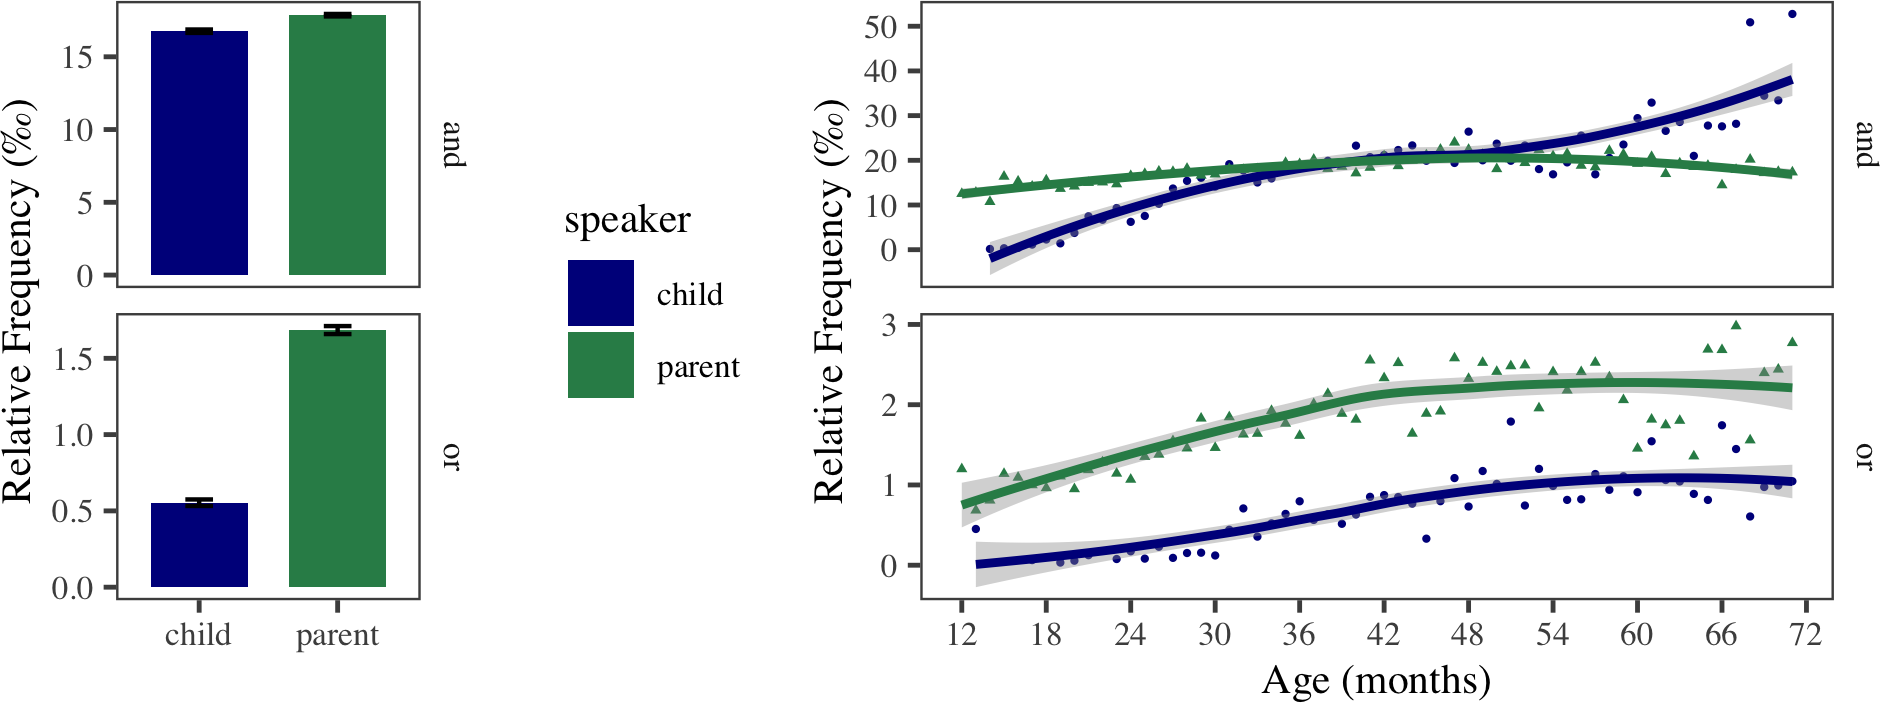
\includegraphics{figs/freqPlots-1} 

}

\caption{Left: The relative frequency of \textit{and/or} (permil) in the speech of parents and children. 95\% binomial proportion confidence intervals calculated using Agresti-Coull's approximate method. Right: The monthly relative frequency of \textit{and/or} (permil) in parents and children's speech between 12 and 72 months (1-6 years).}\label{fig:freqPlots}
\end{figure}

Parental production trends over child age for \emph{and} varied between 10 and 20 uses per 1000 words (Figure \ref{fig:freqPlots}, Right). Children started to produce \emph{and} between 12 and 18 months, with a sharp increase in production until they reached the parent level between 30 to 36 months of age. Child production levels stayed close to their parental levels between 36 and 72 months, possibly even surpassing them at 60 months but the data from 60 months on are sparse.

Parental production of \emph{or} was 1 to 2 per 1000 words. Children started to produce \emph{or} between 18 to 30 months, with increasing uses until they approached 1 use per 1000 words at 48 months (4 years). At this point, their productions plateaued and stayed at this rate through 72 months (6 years). Children started producing \emph{or} about six months later than \emph{and}. While their uses of \emph{and} reached parental levels by around 30 months, their uses of \emph{or} rose more slowly and did not reach the parental level even at age 6.

What factors account for this difference? Previous research has focused on the role of frequency and conceptual complexity (Morris, 2008). First, \emph{and} is far more frequent than \emph{or}. Goodman, Dale, and Li (2008) argued that words from the same syntactic category that are more frequent in child-directed speech are acquired earlier. The conjunction word \emph{and} is at least 10 times more likely to occur than \emph{or} so earlier acquisition of \emph{and} is consistent with the effect of frequency on age of acquisition. Second, research on concept attainment and Boolean concept learning suggests that the concept of conjunction is easier to acquire than disjunction (Feldman, 2000; Neisser \& Weene, 1962; Piantadosi, Tenenbaum, \& Goodman, 2016; Shepard, Hovland, \& Jenkins, 1961). This suggests that children might grasp the concept underlying the meaning of \emph{and} more easily and so produce it early, but need more time to develop the concept underlying the meaning of \emph{or}.

\begin{figure}[H]

{\centering 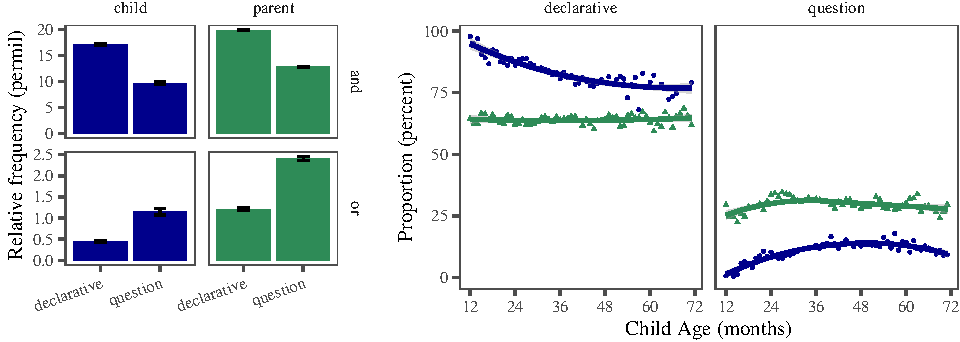
\includegraphics{figs/speechActPlots-1} 

}

\caption{Left: Relative frequency of \textit{and/or} (permil) in declaratives, imperatives, and interrogatives for parents (green) and children (blue). Right: Proportion of declaratives to questions (percent) in parent-child interactions by child-age.}\label{fig:speechActPlots}
\end{figure}

Here we consider a third option: the difference in production between \emph{and} and \emph{or} may be partly due to different patterns in usage. Parent-child interactions are not symmetrical, so the speech acts most favored by parents do not match those favored by young children. This also results in asymmetries in the functional elements used by parents versus children. Child uses of \emph{or} seem to be affected here. First, \emph{or} was more likely to occur in questions than in declaratives (Figure \ref{fig:speechActPlots}, Left). But \emph{and}, in contrast, was more likely to occur in declaratives (Figure \ref{fig:speechActPlots}, Right). Second, parents asked more questions from children than children did from parents. Questions had their own developmental trajectory, emerging in the second year of children's lives and rising to a relatively constant rate of about 15\% of children's utterances in their fourth year. Parents, in comparison, produced questions in about 25\% of their utterances (see also Cameron-Faulkner, Lieven, \& Tomasello, 2003). Therefore, parent-child interaction offers more opportunities for parents to ask questions (and consequently produce \emph{or}), than for children to do so.

\begin{figure}[H]

{\centering 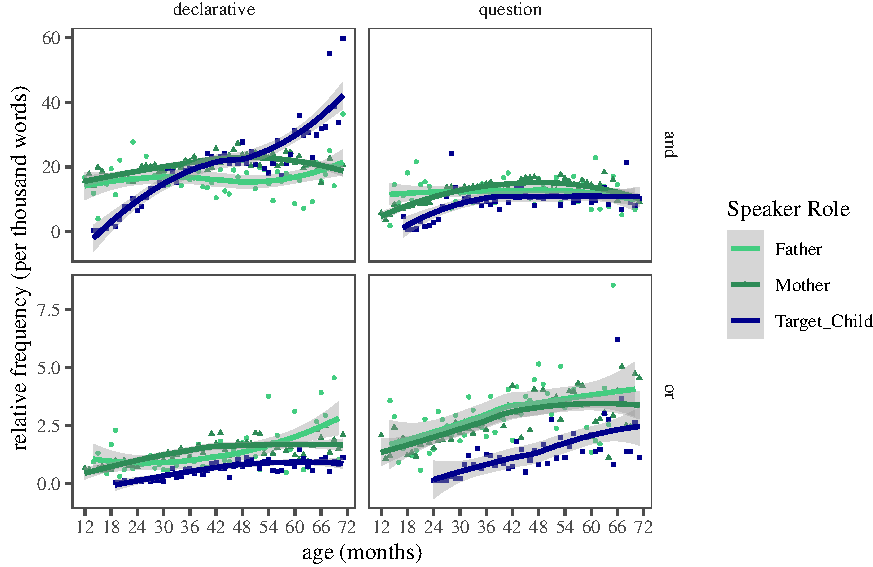
\includegraphics{figs/ageSpeechActPlot-1} 

}

\caption{Relative frequency of \textit{and/or} (permil) in declaratives and questions for parents and childern between the child-age of 12 and 72 months (1-6 years).}\label{fig:ageSpeechActPlot}
\end{figure}

Figure \ref{fig:ageSpeechActPlot} shows the developmental trends for the relative frequencies of \emph{and} and \emph{or} in questions and declaratives. When uses of \emph{and} in these two speech acts are compared, it is clear that the onset of \emph{and} was slightly delayed in questions, but in both utterance types, children reached the parental level by around 30 months (2.5 years). There is a similar delay for \emph{or}: children began producing it in declaratives at around 18 months but not until 24 months in questions. Their production of \emph{or} increased in both declaratives and questions until it reached a constant rate in declaratives between 48 and 72 months. The relative frequency of \emph{or} in questions continued to rise until 60 months. Comparing Figure \ref{fig:freqPlots} and Figure \ref{fig:ageSpeechActPlot}, children were closer to the adult rate of production in declaratives than questions.

To test these observations more formally, we used a multiple linear regression model with the relative frequency of \emph{or} in each monthly time-bin as the dependent variable. The relative frequency was computed by pooling parents' and children's productions across corpora at a given month and dividing the frequency of \emph{or} by the frequency of total words produced in that month by parents or children. Given that there is often very sparse data for each child and corpus, such cross-corpus averaging can help boost signal to noise ratio. Children's age, speaker (child vs.~parent), utterance type (declarative vs.~question), and their interactions served as predictors. The intercept was set to children's productions in declaratives.

Table \ref{tab:study1coeftable} presents the coefficient estimates of the model and Figure \ref{fig:disjunctionPrediction} shows the model fit against the data. This model suggests a significant positive effect of children's age on their production of declarative disjunction (Table \ref{tab:study1coeftable}, ``age'' row). As children grew older, they produced more instances of \emph{or}. The model also estimated significantly higher intercepts for parents producing \emph{or} in declaratives (Table \ref{tab:study1coeftable}, ``parent'' row) as well as questions (parent*question row), which suggests that parents produced more \emph{or} on average than children at the beginning of children's productions. Finally, the model reports a significant interaction of age and utterance type (``age*question'' row), suggesting children increased their production of \emph{or} as they grow older even more in questions, than declaratives. These results are consistent with the hypothesis that frequency and distribution of \emph{or} is partly affected by the production of questions in parent-child interactions.

\begin{table}

\caption{\label{tab:study1coeftable}Estimated cofficients for the linear model with children's age, speaker (child vs. parent), utterance type (declarative vs. question), and their interactions as predictors. Relative frequency of disjunction production was the dependent variable.}
\centering
\fontsize{9}{11}\selectfont
\begin{tabular}[t]{l|r|r|r|r}
\hline
Coefficients & Estimate & Std. Error & t value & Pr(>|t|)\\
\hline
intercept (children, declerative) & 0.0047 & 0.1955 & 0.0242 & 0.9807\\
\hline
age & 0.0188 & 0.0053 & 3.5358 & 0.0005\\
\hline
question & -0.3897 & 0.3022 & -1.2895 & 0.1986\\
\hline
parent & 0.7370 & 0.2452 & 3.0057 & 0.0030\\
\hline
age*question & 0.0319 & 0.0081 & 3.9586 & 0.0001\\
\hline
age*parent & 0.0014 & 0.0069 & 0.2086 & 0.8350\\
\hline
question*parent & 1.2401 & 0.3676 & 3.3736 & 0.0009\\
\hline
age*question*parent & -0.0131 & 0.0101 & -1.2993 & 0.1952\\
\hline
\end{tabular}
\end{table}

\begin{figure}[H]

{\centering 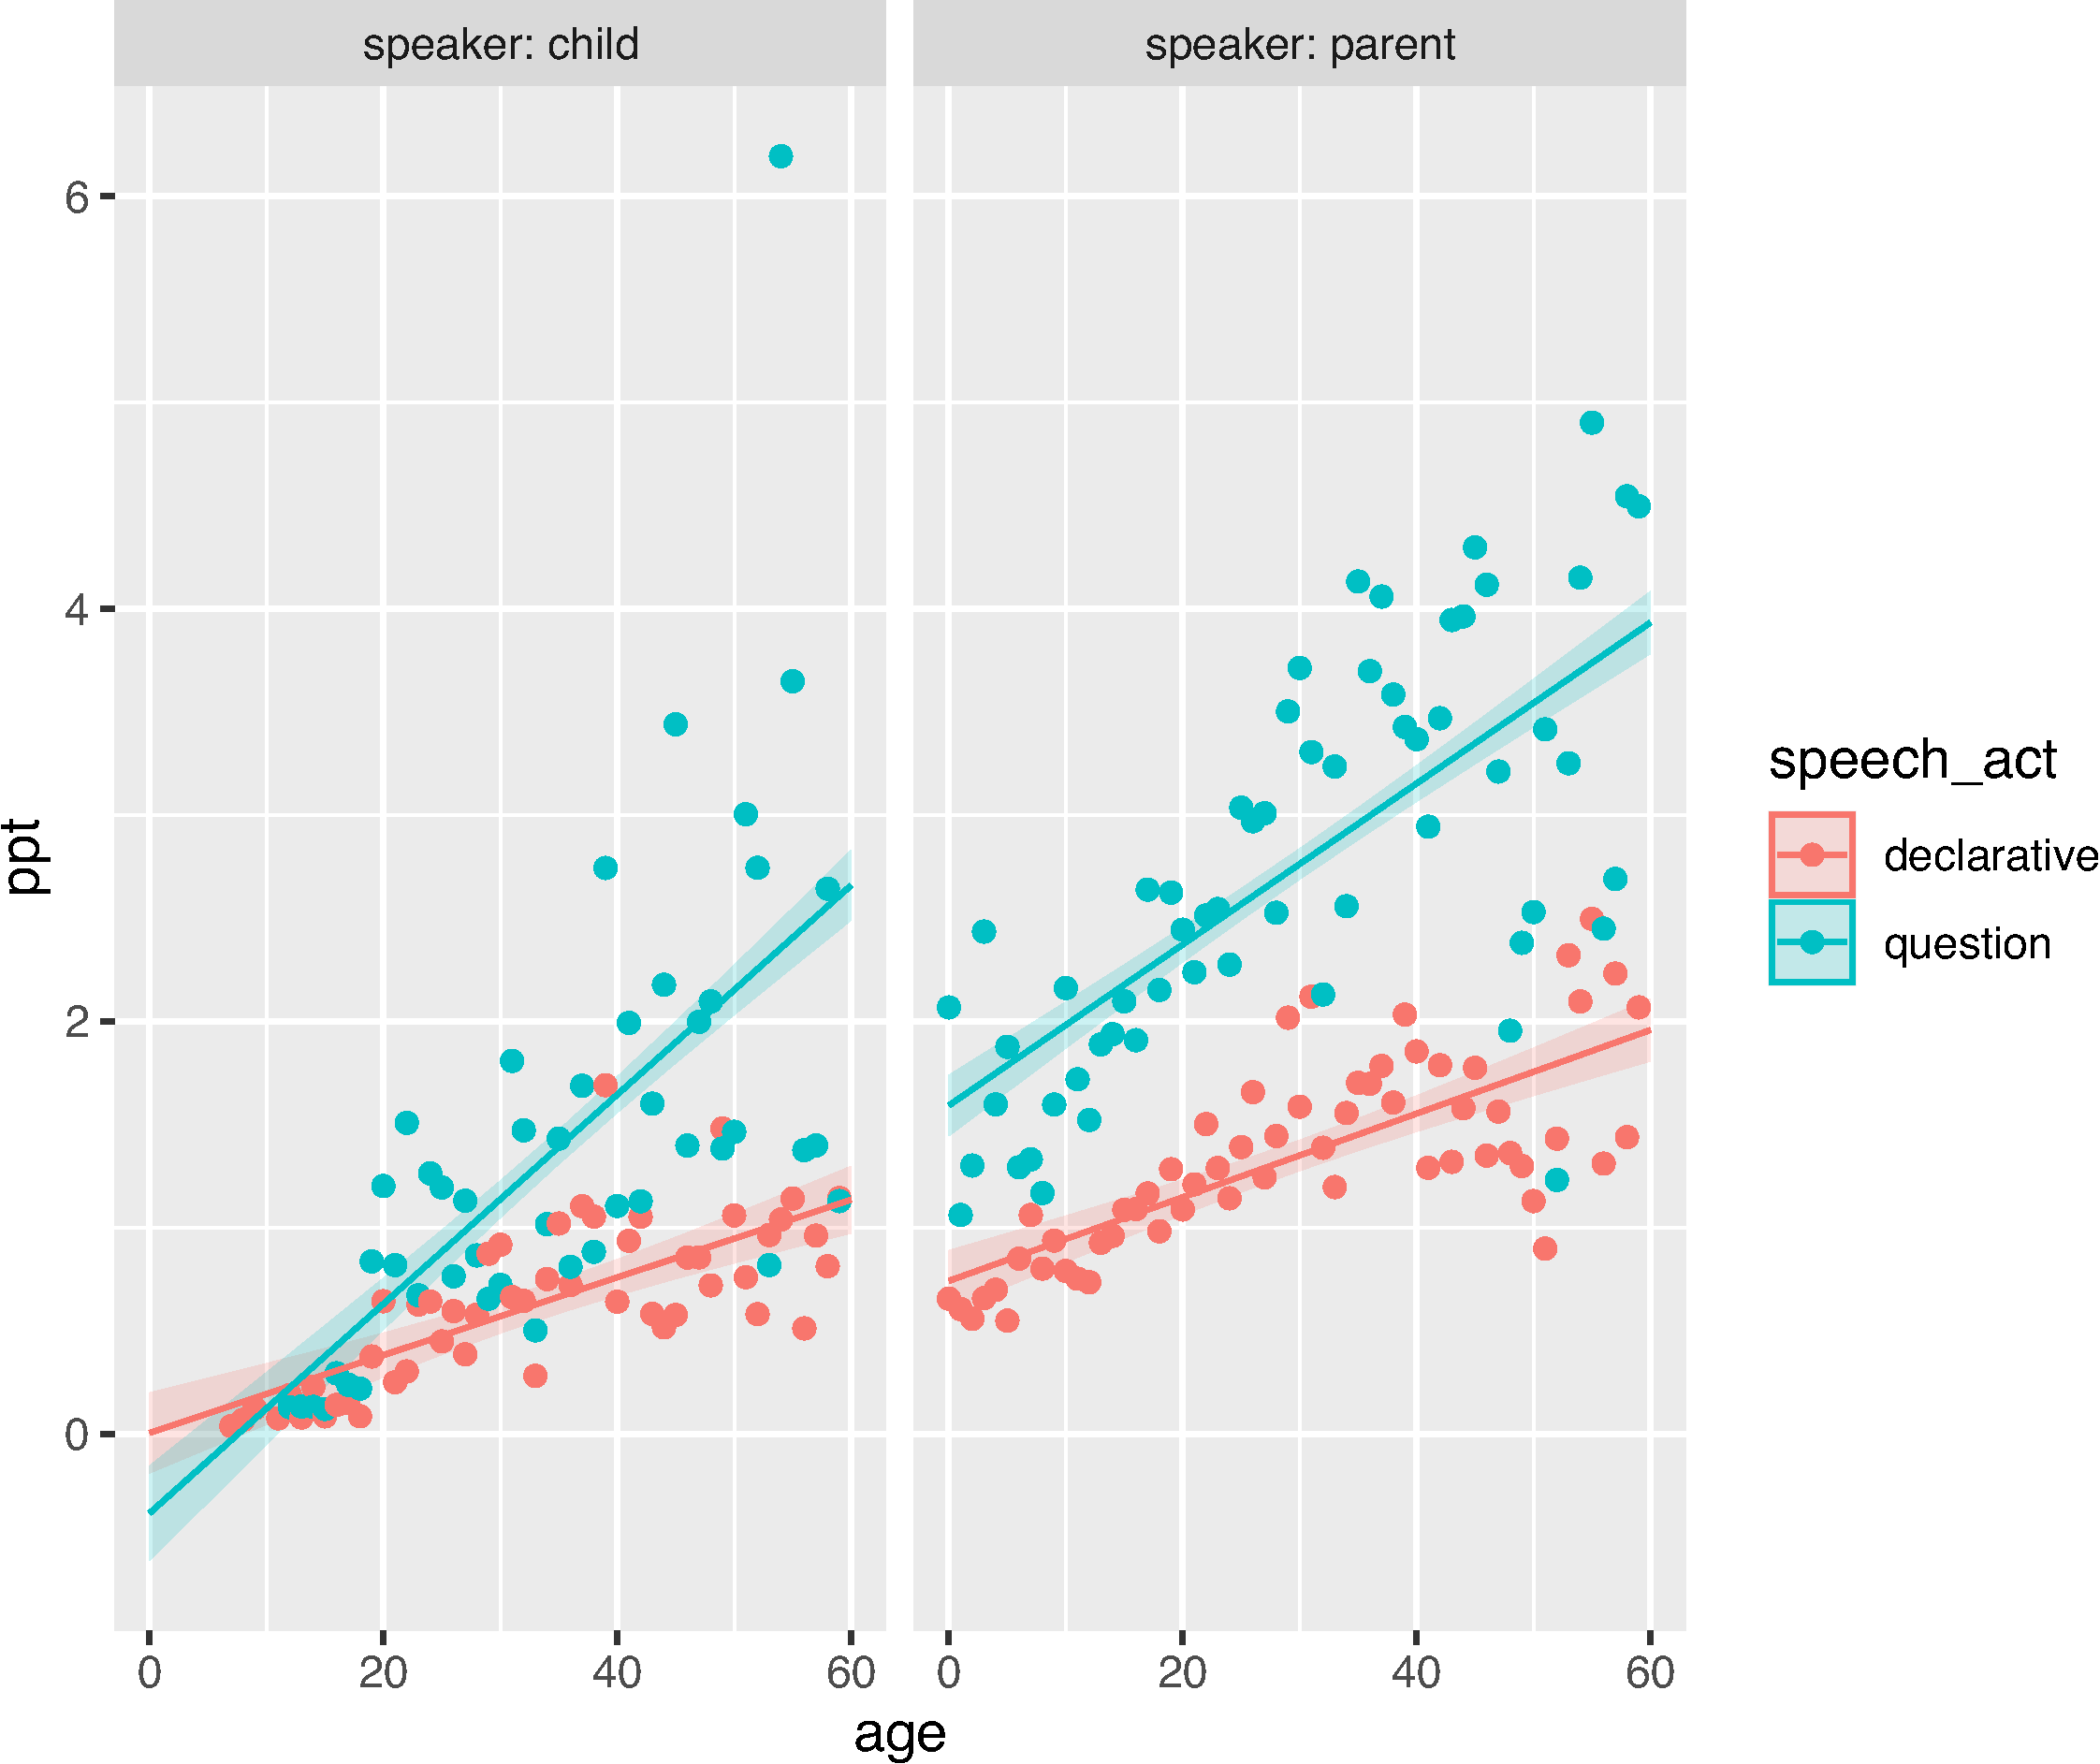
\includegraphics{figs/disjunctionPrediction-1} 

}

\caption{Linear model predictions and the relative frequency of \textit{and/or} (permil) in declaratives and questions for parents and childern between the child-age of 12 (represented as 0 on the x-axis) and 72 months (represented as 60 on the x-axis).}\label{fig:disjunctionPrediction}
\end{figure}

However, there may be considerable variation among children in disjunction production and the model described above does not take this variation into account\footnote{We would like to thank the editor for this comment}. To account for such variation, we fit a separate linear mixed-effects regression model with the relative frequency of \emph{or} in each monthly bin computed separately per child and corpora and used as the dependent variable. The model included random intercepts for corpora and children (nested within corpora), as well as random slopes for age and utterance type (declarative vs.~question). Like the previous model, children's age, speaker (child vs.~parent), utterance type (declarative vs.~question), and their interactions served as predictors and the intercept was set to children's productions of \emph{or} in declaratives.

This mixed-effects model also shows a significant interaction of age and utterance type in children's production of \emph{or} (age*question row), suggesting again that children produce more instances of \emph{or} in questions as they get older compared to declaratives (b = 0.05, t= 2.72, p= 0.01). The model reports the effect of age on children's production of \emph{or} in declaratives is not significant (b = 0.02, t= 1.90, p= 0.06). It also estimated a positive intercept for children's production of \emph{or} in questions compared to declaratives (b = 2.08, t= 2.64, p= 0.01), suggesting that children may start by producing more instances of \emph{or} in questions too. No other effects were significant in this model. Taking both models into account, there is evidence that children's production of disjunction is affected by utterance-type and specifically production of questions in early parent-child interactions.

\hypertarget{study1discussion}{%
\subsection{Conclusion}\label{study1discussion}}

In a large-scale quantitative analysis of parents and children's productions of \emph{and} and \emph{or}, we found that children started producing \emph{and} in the second year of life, and reached parental levels of production by 2;6. Their production of disjunction came about six months later: they started producing \emph{or} between 1;6 and 2;6, arriving at a constant rate around 3;6, but this was at a rate below that of their parents. We suggested some factors that could explain this difference in production such as the frequency or complexity of the connectives. Since parents produced more questions than children, and \emph{or} is more likely to occur in questions, it may be more frequent in parental speech partly because parents ask more questions than children.

\hypertarget{study-2-data-annotation}{%
\section{Study 2: Data Annotation}\label{study-2-data-annotation}}

In this study we focused on the interpretations of a subset of connective examples in child-directed speech from Study 1. Research in formal semantics has shown that the interpretation of disjunction depends on several factors, including prosody (Pruitt \& Roelofsen, 2013), logical consistency of the disjuncts (Geurts, 2006), presence of modals (Kamp, 1973) or negation, and pragmatic reasoning (Grice, 1989). We therefore annotated examples of disjunction for their interpretation, as well as potential cues such as the logical consistency of the disjuncts, the utterance type, the intonation contour, the syntactic category of the disjuncts, the communicative function of the utterance, and the presence or absence of negative or modal morphemes. Since it is difficult to independently verify and annotate for pragmatic reasoning, our study does not identify cases of exclusivity that are due to scalar implicatures (Grice, 1989). However, instances that are not due to any of the factors we have annotated for could potentially be due to scalar implicatures, even though as we shall see, such cases were rare in our dataset.

Our main finding is that in our sample of child-directed speech, exclusive interpretations of \emph{or} are accompanied by rise-fall prosody and logically inconsistent propositions. In the absence of these two properties, \emph{or} is most likely ``not exclusive''. Therefore, these cues could be informative for children with respect to the interpretation of disjunction, and so allow them to partition otherwise inconsistent input. In this section, we provide a descriptive analysis of our annotations without statistical models, leaving statistical modeling for Study 3.

\hypertarget{methods-1}{%
\subsection{Methods}\label{methods-1}}

This study used \href{https://phonbank.talkbank.org/browser/index.php?url=Eng-NA/Providence/}{the Providence corpus} (Demuth, Culbertson, \& Alter, 2006) available from the \href{https://phonbank.talkbank.org}{PhonBank} section of \href{https://talkbank.org/}{TalkBank}. This corpus was chosen because of its relatively dense data on child-directed speech as well as the availability of audio and video recordings that would allow annotators access to the context of the utterance. These data were collected between 2002 and 2005 in Providence, Rhode Island. Table \ref{tab:providence} reports the name, age range, and the number of recording sessions for each child in this study. All the children were monolingual English speakers, followed between the ages of 1 and 4 years, the age range when children develop early understanding of \emph{and} and \emph{or}. The corpus contains 364 hours of biweekly hour-long interactions between parents and children.

\begin{longtable}[]{@{}ccc@{}}
\caption{\label{tab:providence} Information on the participants in the Providence Corpus. Ethan was diagnosed with Asperger's syndrome and therefore was excluded from this study.}\tabularnewline
\toprule()
Name & Age Range & Sessions \\
\midrule()
\endfirsthead
\toprule()
Name & Age Range & Sessions \\
\midrule()
\endhead
Alex & 1;04.28-3;05.16 & 51 \\
Ethan & 0;11.04-2;11.01 & 50 \\
Lily & 1;01.02-4;00.02 & 80 \\
Naima & 0;11.27-3;10.10 & 88 \\
Violet & 1;02.00-3;11.24 & 51 \\
William & 1;04.12-3;04.18 & 44 \\
\bottomrule()
\end{longtable}

\hypertarget{procedure-1}{%
\subsubsection{Procedure}\label{procedure-1}}

We extracted all the utterances containing \emph{and} and \emph{or} using \href{http://alpha.talkbank.org/clan/}{the CLAN software}, with automatic tagging for the following: (1) the name of the child; (2) the transcript address; (3) the speaker of the utterance (father, mother, or child); (4) the child's birth date, and (5) the recording date. Since the focus of this study was on disjunction, we annotated instances of \emph{or} in child-directed speech from the earliest examples to the latest ones. Since the corpus contained more than 10 times the number of \emph{and} than of \emph{or}, we randomly sampled 1000 examples of \emph{and} to match 1000 examples of \emph{or} in the same age range. After checking for inter-rater reliability, we annotated and analyzed 608 examples of \emph{or} and 627 examples of \emph{and} in the allotted time for annotations.

\hypertarget{annotation-categories}{%
\subsubsection{Annotation Categories}\label{annotation-categories}}

Every extracted instance of \emph{and} and \emph{or} was manually annotated for eight properties: 1. connective interpretation, 2. logical consistency, 3. utterance type, 4. intonation type, 5. syntactic level, 6. communicative function, 7. answer type, and 8. negation and modals. Below we briefly explain how each annotation was defined. Further details and examples are given in the appendix.

\begin{enumerate}
\def\labelenumi{\arabic{enumi}.}
\tightlist
\item
  \emph{Connective Interpretation}
\end{enumerate}

This annotation category was the dependent variable in this study. Annotators listened to utterances such as ``A or B'' and ``A and B'', and decided on the intended interpretation with respect to the truth of propositions A and B. We considered 16 possible binary connective meanings. Table \ref{tab:connectiveInterpretaion} shows the most common connective meanings we found in child-directed speech with some examples. Annotators were asked to consider the two propositions (A and B) in the coordinated structure, ignoring the connective and functional elements such as negation. Consider: ``Bob plays soccer or tennis'' and ``Bob doesn't play soccer or tennis''. Both contain the same two propositions: A. Bob playing soccer, and B. Bob playing tennis, but the functional elements that combine the two propositions (namely \emph{or} and \emph{doesn't}) result in different interpretations with respect to the truth of A and B. In ``Bob plays soccer or tennis'', which contains a disjunction, the interpretation is that Bob plays one or possibly both sports (i.e.~inclusive disjunction annotated as IOR). In ``Bob doesn't play soccer or tennis'', which contains a negation and a disjunction, the interpretation is that Bob plays neither sport (NOR).

In a different sentence like ``Bob drank coffee or tea this morning'', the dominant interpretation is that he drank one or the other, but not both (i.e.~exclusive disjunction annotated as XOR). However, sometimes disjunction is used to provide a conversational repair. Consider ``Bob drank coffee, or I mean, tea this morning.'' In such cases the speaker intends the second proposition as true and the first is false or not intended. We annotated such cases as NAB. A very common interpretation for both conjunction and disjunction is that both propositions are true (AND). Consider this example with \emph{or}: ``Bob plays sports like soccer or tennis''. Here the intended meaning is that Bob plays both sports. Notice that in this example changing the connective from \emph{or} to \emph{and} creates no change in the intended meaning: ``Bob plays sports like soccer and tennis.'' Another interpretation attested in our sample of child directed speech was one in which the speaker conveys that both propositions are not true but one or the other could be true, and possibly neither (NAND). For example, if someone says ``I do not like peanut butter and jelly'', they may still like one without the other or possibly like neither. Finally, sometimes a connective can convey that one proposition is true if and only if the other is true. For example, a mother may say ``come here and I'll show you'' which can be equivalent to: if and only of you come here, I'll show you. We annotated such cases as IFF. For all annotations of connective interpretations, the annotators first reconstructed the coordinated propositions without the connectives or negation, and then decided which propositions were implied to be true/false.

\begin{longtable}[]{@{}
  >{\raggedright\arraybackslash}p{(\columnwidth - 4\tabcolsep) * \real{0.0641}}
  >{\raggedright\arraybackslash}p{(\columnwidth - 4\tabcolsep) * \real{0.3974}}
  >{\raggedright\arraybackslash}p{(\columnwidth - 4\tabcolsep) * \real{0.5385}}@{}}
\caption{\label{tab:connectiveInterpretaion} Annotation classes for connective interpretation}\tabularnewline
\toprule()
\begin{minipage}[b]{\linewidth}\raggedright
Class
\end{minipage} & \begin{minipage}[b]{\linewidth}\raggedright
Meaning
\end{minipage} & \begin{minipage}[b]{\linewidth}\raggedright
Examples
\end{minipage} \\
\midrule()
\endfirsthead
\toprule()
\begin{minipage}[b]{\linewidth}\raggedright
Class
\end{minipage} & \begin{minipage}[b]{\linewidth}\raggedright
Meaning
\end{minipage} & \begin{minipage}[b]{\linewidth}\raggedright
Examples
\end{minipage} \\
\midrule()
\endhead
AND & Both propositions are true & \emph{``I'm just gonna empty this and then I'll be out of the kitchen.'' -- ``I'll mix them together or I could mix it with carrot, too.''} \\
IOR & One or both propositions are true & \emph{``You should use a spoon or a fork.'' -- ``Ask a grownup for some juice or water or soy milk.''} \\
XOR & Only one proposition is true & \emph{``Is that a hyena? or a leopard?'' -- ``We're gonna do things one way or the other.''} \\
NOR & Neither proposition is true & \emph{``I wouldn't say boo to one goose or three.'' -- ``She found she lacked talent for hiding in trees, for chirping like crickets, or humming like bees.''} \\
NAND & It's not the case that both propositions are true. & \emph{I do not like green eggs and ham -- you don't swing that in the house and hit things with it} \\
IFF & Either both propositions are true or both are false & \emph{``Put them {[}crayons{]} up here and you can get down. -- Come over here and I'll show you.''} \\
NAB & The first proposition is false, the second is true. & \emph{``There's an Oatio here, or actually, there's a wheat here.''} \\
\bottomrule()
\end{longtable}

\begin{enumerate}
\def\labelenumi{\arabic{enumi}.}
\setcounter{enumi}{1}
\tightlist
\item
  \emph{Logical Consistency}
\end{enumerate}

Propositions can have logical, temporal, or causal relations with each other. For logical consistency, annotators decided whether the propositions in each coordination could be true at the same time or not. If they could not, because that would result in a contradiction, they were marked as inconsistent (Table \ref{tab:consistencyType}). The annotations used the following diagnostic here: Two disjuncts were inconsistent if replacing the word \emph{or} with \emph{and} resulted in a contradiction. For example, changing ``the ball is in my room \emph{or} your room'' to ``the ball is in my room \emph{and} your room'' produces a contradiction because a ball cannot be in two rooms at once.

Two issues arise with respect to logical consistency. First, our diagnostic is quite strict. In many cases, propositions are not inconsistent so much as implausible. For example, drinking both tea and coffee at the same time is consistent, but not conventionally likely or plausible. Many exclusive interpretations may be based on such judgments of plausibility. Second, if the coordinands are inconsistent, this does not necessarily mean that the connective interpretation must be exclusive. For example, in ``you could stay here or go out'', the alternatives ``staying here'' and ``going out'' are inconsistent, yet the overall interpretation of the connective could still be conjunctive: you could stay here AND you could go out. Both possibilities hold. This pattern of interaction between possibility modals like \emph{can} and disjunctive terms like \emph{or} are often discussed as ``free-choice inferences'' in the semantics and pragmatics literature (Kamp, 1973; Von Wright, 1968). Another example is unconditionals such as ``Ready or not, here I come!''. The coordinands are contradictions: one is the negation of the other. But the overall interpretation is that, in both cases, the speaker is going to come.

\begin{longtable}[]{@{}
  >{\raggedright\arraybackslash}p{(\columnwidth - 4\tabcolsep) * \real{0.1639}}
  >{\raggedright\arraybackslash}p{(\columnwidth - 4\tabcolsep) * \real{0.3115}}
  >{\raggedright\arraybackslash}p{(\columnwidth - 4\tabcolsep) * \real{0.5246}}@{}}
\caption{\label{tab:consistencyType} Definitions of consistency types and their examples.}\tabularnewline
\toprule()
\begin{minipage}[b]{\linewidth}\raggedright
Consistency
\end{minipage} & \begin{minipage}[b]{\linewidth}\raggedright
Definitions
\end{minipage} & \begin{minipage}[b]{\linewidth}\raggedright
Examples
\end{minipage} \\
\midrule()
\endfirsthead
\toprule()
\begin{minipage}[b]{\linewidth}\raggedright
Consistency
\end{minipage} & \begin{minipage}[b]{\linewidth}\raggedright
Definitions
\end{minipage} & \begin{minipage}[b]{\linewidth}\raggedright
Examples
\end{minipage} \\
\midrule()
\endhead
Consistent & The coordinands can be true at the same time. & \emph{``We could spell some things with a pen or draw some pictures.''} \\
Inconsistent & The coordinands cannot be true at the same time. & \emph{``Do you want to stay or go?''} \\
\bottomrule()
\end{longtable}

\begin{enumerate}
\def\labelenumi{\arabic{enumi}.}
\setcounter{enumi}{2}
\tightlist
\item
  \emph{Utterance Type}
\end{enumerate}

Annotators decided whether an utterance was an instance of a declarative, an interrogative, or an imperative. We occasionally found examples with different utterance types for each coordinand. A mother might say ``put your backpack on and I'll be right back'', where the first coordinand is an imperative and the second a declarative. These were coded for both utterance types with a dash in between: imperative-declarative. Table \ref{tab:utteranceTypes} in the appendix provides the detailed definitions and examples for each utterance type.

\begin{longtable}[]{@{}
  >{\raggedright\arraybackslash}p{(\columnwidth - 4\tabcolsep) * \real{0.1923}}
  >{\raggedright\arraybackslash}p{(\columnwidth - 4\tabcolsep) * \real{0.4615}}
  >{\raggedright\arraybackslash}p{(\columnwidth - 4\tabcolsep) * \real{0.3462}}@{}}
\caption{\label{tab:utteranceTypes} Definitions of the utterance types and their examples.}\tabularnewline
\toprule()
\begin{minipage}[b]{\linewidth}\raggedright
Utterance Types
\end{minipage} & \begin{minipage}[b]{\linewidth}\raggedright
Definitions
\end{minipage} & \begin{minipage}[b]{\linewidth}\raggedright
Examples
\end{minipage} \\
\midrule()
\endfirsthead
\toprule()
\begin{minipage}[b]{\linewidth}\raggedright
Utterance Types
\end{minipage} & \begin{minipage}[b]{\linewidth}\raggedright
Definitions
\end{minipage} & \begin{minipage}[b]{\linewidth}\raggedright
Examples
\end{minipage} \\
\midrule()
\endhead
Declarative & A statement with a subject-verb-object word order and a flat intonation. & \emph{``It looks a little bit like a drum stick or a mallet.''} \\
Interrogative & A question with either subject-auxiliary inversion or a rising terminal intonation. & \emph{``Is that a dog or a cat?''} \\
Imperative & A directive with an uninflected verb and no subject & \emph{``Have a little more French toast or have some of your juice.''} \\
\bottomrule()
\end{longtable}

\begin{enumerate}
\def\labelenumi{\arabic{enumi}.}
\setcounter{enumi}{3}
\tightlist
\item
  \emph{Intonation Type}
\end{enumerate}

Annotators listened to the utterances and decided whether the intonation contour was flat, rise, or rise-fall. Table \ref{tab:intonationTypes} in the appendix gives the definitions and examples for these intonation types. In order to judge the intonation of an utterance accurately, annotators were asked to construct all three intonation contours for the same utterance from transcriptions and see which one matched the actual intonation in the video recordings. For example, to judge ``do you want orange juice\(\uparrow\) or apple juice\(\downarrow\)?'', they reconstructed the sentence with the prototypical flat, rising, and rise-fall intonations and checked to see which was closer to the actual contour.

\begin{longtable}[]{@{}
  >{\raggedright\arraybackslash}p{(\columnwidth - 4\tabcolsep) * \real{0.1176}}
  >{\raggedright\arraybackslash}p{(\columnwidth - 4\tabcolsep) * \real{0.5000}}
  >{\raggedright\arraybackslash}p{(\columnwidth - 4\tabcolsep) * \real{0.3824}}@{}}
\caption{\label{tab:intonationTypes} Definitions of the intonation types and their examples.}\tabularnewline
\toprule()
\begin{minipage}[b]{\linewidth}\raggedright
Intonation
\end{minipage} & \begin{minipage}[b]{\linewidth}\raggedright
Definitions
\end{minipage} & \begin{minipage}[b]{\linewidth}\raggedright
Examples
\end{minipage} \\
\midrule()
\endfirsthead
\toprule()
\begin{minipage}[b]{\linewidth}\raggedright
Intonation
\end{minipage} & \begin{minipage}[b]{\linewidth}\raggedright
Definitions
\end{minipage} & \begin{minipage}[b]{\linewidth}\raggedright
Examples
\end{minipage} \\
\midrule()
\endhead
Flat & Intonation does not show any substantial rise at the end of the sentence. & \emph{``I don't hear any meows or bow-wow-wows.''} \\
Rise & There is a substantial intonation rise on each disjunct or generally on both. & \emph{``Do you want some seaweed? or some wheat germ?''} \\
Rise-Fall & There is a substantial rise on the non-final disjunct(s), and a fall on the final disjunct. & \emph{``Is that big Q or little q?'' -- ``(are) You patting them, petting them, or slapping them?''} \\
\bottomrule()
\end{longtable}

\begin{enumerate}
\def\labelenumi{\arabic{enumi}.}
\setcounter{enumi}{4}
\tightlist
\item
  \emph{Syntactic Level}
\end{enumerate}

Annotators marked whether the coordination was at the clausal level or sub-clausal level (Table @ref\label{tab:syntacticLevel}). Clausal level was defined as sentences, clauses, verb phrases, and verbs. Coordination of other categories was coded as sub-clausal. This annotation category was introduced to check whether the syntactic category of the coordinands influenced the interpretation of a coordination. For example, ``He drank tea or coffee'' is less likely to be interpreted as exclusive than ``He drank tea or he drank coffee.'' The clausal vs.~sub-clausal distinction was inspired by the fact that in many languages, coordinators that connect sentences and verb phrases differ from those that connect nominal, adjectival, or prepositional phrases (Haspelmath, 2007).

\begin{longtable}[]{@{}
  >{\raggedright\arraybackslash}p{(\columnwidth - 4\tabcolsep) * \real{0.1852}}
  >{\raggedright\arraybackslash}p{(\columnwidth - 4\tabcolsep) * \real{0.4074}}
  >{\raggedright\arraybackslash}p{(\columnwidth - 4\tabcolsep) * \real{0.4074}}@{}}
\caption{\label{tab:syntacticLevel} Definitions of the syntactic levels and their examples.}\tabularnewline
\toprule()
\begin{minipage}[b]{\linewidth}\raggedright
Syntactic Level
\end{minipage} & \begin{minipage}[b]{\linewidth}\raggedright
Definitions
\end{minipage} & \begin{minipage}[b]{\linewidth}\raggedright
Examples
\end{minipage} \\
\midrule()
\endfirsthead
\toprule()
\begin{minipage}[b]{\linewidth}\raggedright
Syntactic Level
\end{minipage} & \begin{minipage}[b]{\linewidth}\raggedright
Definitions
\end{minipage} & \begin{minipage}[b]{\linewidth}\raggedright
Examples
\end{minipage} \\
\midrule()
\endhead
Clausal & The coordinands are sentences, clauses, verb phrases, or verbs. & \emph{``Does he lose his tail sometimes and Pooh helps him and puts it back on?''} \\
Sub-clausal & The coordinands are nouns, adjectives, noun phrases, determiner phrases, or prepositional phrases. & \emph{``Hollies can be bushes or trees.''} \\
\bottomrule()
\end{longtable}

\begin{enumerate}
\def\labelenumi{\arabic{enumi}.}
\setcounter{enumi}{5}
\tightlist
\item
  \emph{Communicative Functions}
\end{enumerate}

We constructed a set of categories to capture particular usages or communicative functions of the words \emph{or} and \emph{and}. These included descriptions, directives, preferences, identifications, definitions-examples, clarifications, repairs (see Appendix, Table \ref{tab:speechActs}. These communicative functions were created using the first 100 examples, then used for the classifications of all the rest. Some are general and some specific to coordination. For example, directives are general while conditionals (e.g.~Put that out of your mouth, or I'm gonna put it away) are more specific to coordinated constructions. Our list was not unstructured: some communicative functions are subtypes of others. For instance, ``identifications'' and ``unconditionals'' are subtypes of ``descriptions'' while ``conditionals'' are a subtype of directives. Furthermore, ``repairs'' seem parallel to other categories in that any type of speech can be repaired. Such details will matter for any general theory of acquisition where the speaker's communicative intentions offer cues for the eventual acquisition of function words.

\begin{longtable}[]{@{}
  >{\raggedright\arraybackslash}p{(\columnwidth - 4\tabcolsep) * \real{0.1444}}
  >{\raggedright\arraybackslash}p{(\columnwidth - 4\tabcolsep) * \real{0.4889}}
  >{\raggedright\arraybackslash}p{(\columnwidth - 4\tabcolsep) * \real{0.3667}}@{}}
\caption{\label{tab:speechActs} Definitions of the communicative functions and their examples.}\tabularnewline
\toprule()
\begin{minipage}[b]{\linewidth}\raggedright
Function
\end{minipage} & \begin{minipage}[b]{\linewidth}\raggedright
Definitions
\end{minipage} & \begin{minipage}[b]{\linewidth}\raggedright
Examples
\end{minipage} \\
\midrule()
\endfirsthead
\toprule()
\begin{minipage}[b]{\linewidth}\raggedright
Function
\end{minipage} & \begin{minipage}[b]{\linewidth}\raggedright
Definitions
\end{minipage} & \begin{minipage}[b]{\linewidth}\raggedright
Examples
\end{minipage} \\
\midrule()
\endhead
Descriptions & Describing what the world is like or asking about it. The primary goal is to inform the addressee about how things are. & ``\emph{It's not in the ditch or the drain pipe.}'' \\
Identifications & Identifying the category membership or an attribute of an object. Speaker has uncertainty. A subtype of ``Description''. & ``\emph{Is that a ball or a balloon honey?}'' \\
Definitions and Examples & Providing labels for a category or examples for it. Speaker is certain. Subtype of Description. & \emph{``This is a cup or a mug.'' -- ``berries like blueberry or raspberry''} \\
Preferences & Asking what the addressee wants or would like or stating what the speaker wants or would like & \emph{``Do you wanna play pizza or read the book?''} \\
Options & Either asking or listing what one can or is allowed to do. Giving permission, asking for permission, or describing the possibilities. Often the modal ``can'' is either present or can be inserted. & \emph{``You could have wheat or rice.''} \\
Directives & Directing the addressee to act or not act in a particular way. Common patterns include ``let's do \ldots{}'', ``Why don't you do \ldots{}'', or prohibitions such as ``Don't \ldots{}''. The difference with ``options'' is that the speaker expects the directive to be carried out by the addressee. There is no such expectation for ``options''. & \emph{``let's go back and play with your ball or we'll read your book.''} \\
Clarifications & Something is said or done as a communicative act but the speaker has uncertainty with respect to the form or the content. & \emph{``You mean boba or bubble?''} \\
Repairs & Speaker correcting herself on something she said (self repair) or correcting the addressee (other repair). The second disjunct is what holds and is intended by the speaker. The speaker does not have uncertainty with respect to what actually holds. & \emph{``There's an Oatio here, or actually, there's a wheat here.''} \\
Conditionals & Explaining in the second coordinand, what would follow if the first coordinand is (or is not) followed. Subtype of Directive. & \emph{``Put that out of your mouth, or I'm gonna put it away.''} -- \emph{``Come over here and I'll show you.''} \\
Unconditionals & Denying the dependence of something on a set of conditions. Typical format: ``Whether X or Y, Z''. Subtype of Descriptions. & \emph{``Ready or not, here I come!''} (playing hide and seek) \\
\bottomrule()
\end{longtable}

\begin{enumerate}
\def\labelenumi{\arabic{enumi}.}
\setcounter{enumi}{6}
\tightlist
\item
  \emph{Answer Type}
\end{enumerate}

Whenever a parent's utterance was a polar question, annotators coded for the type of response it received from the children. This category was different from others because it was not a potential cue for learning disjunction. Instead, it offered an opportunity to assess (in a limited, conservative manner) children's comprehension within the corpus data. Table \ref{tab:answerTypes} (Appendix) gives the answer types in this study, along with definitions and examples. Utterances that were not polar questions were simply coded as NA. If children responded to polar questions with ``yes'' or ``no'', the category was YN, and if they repeated one of the coordinands, the category was AB. If children said yes/no and followed it with one of the coordinands, the answer type was determined as YN (yes/no). For example, if a child was asked ``Do you want orange juice or apple juice?'' and the child responded with ``yes, apple juice'', our annotators coded the response as YN, because in almost all cases, if simple yes/no is felicitous, then it can also be followed (optionally) with one of the disjunct. But, if yes/no is not a felicitous response, then mentioning one of the disjuncts is the only appropriate answer. For example, if someone asks ``Do you want to stay here or go out?'' a response such as ``yes, go out'' is infelicitous; a better response is simply ``go out''. We therefore counted responses with both yes/no and mention of a disjunct as a yes/no response. We did not annotate for non-verbal answers like head nods or head shakes. This is therefore a limited and conservative measure of children's comprehension of disjunctive questions.

\begin{longtable}[]{@{}
  >{\raggedright\arraybackslash}p{(\columnwidth - 4\tabcolsep) * \real{0.1857}}
  >{\raggedright\arraybackslash}p{(\columnwidth - 4\tabcolsep) * \real{0.4571}}
  >{\raggedright\arraybackslash}p{(\columnwidth - 4\tabcolsep) * \real{0.3571}}@{}}
\caption{\label{tab:answerTypes} Definitions of answer types and their examples.}\tabularnewline
\toprule()
\begin{minipage}[b]{\linewidth}\raggedright
Type
\end{minipage} & \begin{minipage}[b]{\linewidth}\raggedright
Definitions
\end{minipage} & \begin{minipage}[b]{\linewidth}\raggedright
Examples
\end{minipage} \\
\midrule()
\endfirsthead
\toprule()
\begin{minipage}[b]{\linewidth}\raggedright
Type
\end{minipage} & \begin{minipage}[b]{\linewidth}\raggedright
Definitions
\end{minipage} & \begin{minipage}[b]{\linewidth}\raggedright
Examples
\end{minipage} \\
\midrule()
\endhead
No Answer & The child provides no answer to the question. & Mother: \emph{``Would you like to eat some applesauce or some carrots?''} Child: \emph{``Guess what Max!''} \\
YN & The child responds with \emph{yes} or \emph{no}. & Father: \emph{``Can I finish eating one or two more bites of my cereal?''} Child: \emph{``No.''} \\
AB & The child responds with one of the disjuncts (alternatives). & Mother: \emph{``Is she a baby elephant or is she a toddler elephant?''} Child: \emph{``It's a baby. She has a tail.''} \\
\bottomrule()
\end{longtable}

\begin{enumerate}
\def\labelenumi{\arabic{enumi}.}
\setcounter{enumi}{7}
\tightlist
\item
  \emph{Negation and Modals}
\end{enumerate}

Finally, was used a script to automatically mark utterances that contained sentential negation (\emph{not}/\emph{n't}) or any modal element such as \emph{maybe}, \emph{can}, \emph{could}, \emph{should}, \emph{would}, or \emph{need to}. This allowed us to see whether the presence or absence of negation or modals affected the overall interpretation of the utterance.

\hypertarget{inter-annotator-reliability}{%
\subsubsection{Inter-annotator Reliability}\label{inter-annotator-reliability}}

To train annotators and assess their reliability, two annotators coded the same 240 instances of disjunction. Their reliability was calculated over eight iterations of 30 examples each. After each iteration, annotators met to discuss and resolve disagreements. They also decided whether to make category definitions or annotation criteria more precise. Training was completed after three consecutive iterations showed substantial agreement for all categories (Cohen's \(\kappa > 0.7\)) (for further details, see the Appendix).

\hypertarget{exclusion-criteria-1}{%
\subsubsection{Exclusion Criteria}\label{exclusion-criteria-1}}

We excluded one child (Ethan) from the Providence corpus, given his diagnosis of Asperger's Syndrome at age 5. We also excluded all examples from conversations over the phone, in adult-adult exchanges, and in utterances heard from TV or radio. Such utterances were not counted as child-directed speech. We also excluded proper names and fixed forms like ``Bread and Circus'' (name of a local place) or ``trick-or-treat'' from the set of examples to be annotated. Such forms could be learned as chunks with no actual understanding of the connective meaning. We counted multiple instances of \emph{or} and \emph{and} with the same disjunction/conjunction as one instance. Our reasoning was that, in a coordinated structure, the additional occurrences of a connective typically did not alter the annotation categories nor the interpretation of the coordination. For example, there is little difference between ``cat, dog, and elephant'' versus ``cat and dog and elephant'' in interpretation. Our focus was on the ``coordinated construction'' as a unit rather than on every separate instance of \emph{and} and \emph{or}. Instances of multiple connectives in a coordination were rare.

\hypertarget{results}{%
\subsection{Results}\label{results}}

We start with ``answer types''. This category provides some measure of children's comprehension by showing when children provide appropriate answers to questions containing a disjunction. We then look at our dependent variable, namely the ``connective interpretations'', and then move on to the cues that potentially aid the acquisition of connective interpretations.

\hypertarget{answer-types}{%
\subsubsection{Answer Types}\label{answer-types}}

Figure \ref{fig:answerPlot} (Left) shows the monthly proportions of ``yes/no'' (Y/N) and alternative (AB) answers between the ages of 1 and 3 years. At first, children provided no answers, but by the age 3, they gave a yes/no (YN) or alternative (AB) answer to most polar questions. To assess how often their answers were appropriate, we defined as appropriate answer the following: an alternative (AB) answer was appropriate for an alternative question (one with ``or'' and rise-fall intonation). A yes/no answer (YN) is appropriate for a yes/no (polar) question (one with \emph{or} and a rising intonation). This strict classification misses some nuanced cases, but it provides a useful, if conservative, estimate of comprehension. Figure \ref{fig:answerPlot} (Right) shows the monthly proportion of children's appropriate answers between the ages of 1 and 3. Children offered an increasing number of appropriate answers to questions containing \emph{or} between 20 to 30 months of age. This suggests that they form initial mappings for the meaning of disjunction in this age range. We now turn to cues that could assist children in making successful mappings for disjunctive meanings.

\begin{figure}[H]

{\centering 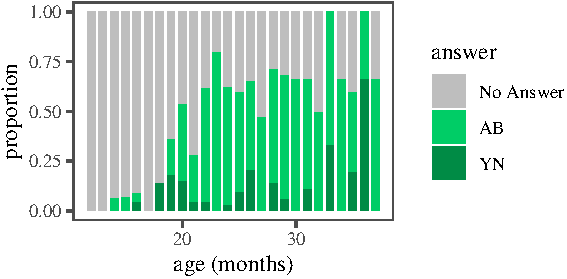
\includegraphics{figs/answerPlot-1} 

}

\caption{Left: Monthly proportions of children's yes/no (YN) and alternative (AB) answers to questions with \textit{or}. Right: Monthly proportions of children's appropriate answers to questions with \textit{or}.}\label{fig:answerPlot}
\end{figure}

\hypertarget{connective-interpretation}{%
\subsubsection{Connective Interpretation}\label{connective-interpretation}}

\begin{figure}[H]

{\centering 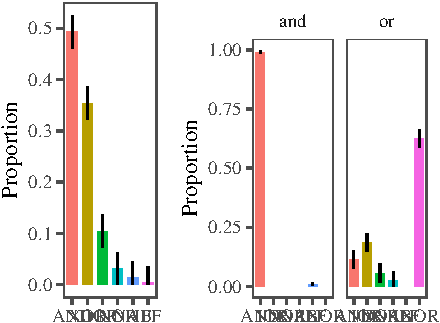
\includegraphics{figs/interpretationPlot-1} 

}

\caption{Connective Interpretations broken down by lexical items \textit{and} (conjunction) and \textit{or} (disjunction).}\label{fig:interpretationPlot}
\end{figure}

Regardless of the connective word used, the most common interpretation was conjunction (AND, 55\%) followed by exclusive disjunction (XOR, 31\%). Figure \ref{fig:interpretationPlot} shows the distribution of connective interpretations according to the connective term -- \emph{and} vs.~\emph{or}\footnote{All the confidence intervals shown in the plots for this section are simultaneous multinomial confidence intervals computed using the Sison and Glaz (1995) method.} (\(N_{and}\) = 627 utterances, \(N_{or}\) = 608 utterances). Almost all instances of the connective \emph{and}, were interpreted as conjunction (AND). There were also a small number of NAND interpretations (e.g.~``don't swing that in the house and hit things with it'') and IFF interpretations (e.g.~``come here and I'll show you'') in the sample. For the connective \emph{or}, the most frequent interpretation was exclusive disjunction (XOR, 62\%) followed by inclusive disjunction (IOR, 18\%) and conjunction (AND, 11\%). There were also a small number of NOR (e.g.~``you never say goodbye or thank you'') and NAB interpretations (e.g.~``those screws, or rather, those nuts''). Overall, these results are consistent with the findings of Morris (2008) who concluded that exclusive disjunction is the most common interpretation of \emph{or} in child-directed speech. Therefore, by simply associating the most common interpretations with the connective words, learners are expected to acquire \emph{and} as conjunction, and \emph{or} as exclusive disjunction (Crain, 2012; Morris, 2008). However, the learning outcome might be different if factors other than the connective word are also taken into account. In the next section, we look at how different annotation categories accompany the interpretations of \emph{or}.

\hypertarget{cues-to-disjunction-interpretation}{%
\subsubsection{Cues to Disjunction Interpretation}\label{cues-to-disjunction-interpretation}}

\begin{figure}[H]

{\centering 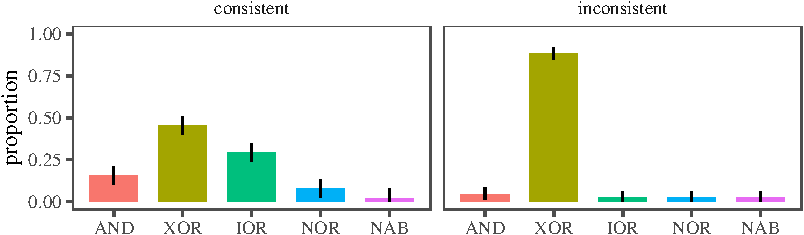
\includegraphics{figs/consistencyPlot-1} 

}

\caption{Interpretations of disjunction in child-directed speech with consistent vs. inconsistent disjuncts.}\label{fig:consistencyPlot}
\end{figure}

We set \emph{and} aside because it was nearly always interpreted as conjunction (AND). Figure \ref{fig:consistencyPlot} shows the proportions of connective interpretations in disjunctions with consistent (N=364 utterances) vs.~inconsistent disjuncts (N=244 utterances). When the disjuncts were consistent (i.e.~could be true at the same time), the interpretation could be exclusive (XOR), inclusive (IOR), or conjunctive (AND). When the disjuncts were inconsistent, a disjunction almost always received an exclusive (XOR) interpretation. This suggests that the exclusive interpretation of a disjunction often stems from the inconsistent or contradictory nature of the disjuncts themselves\footnote{It should be noted here that in all \emph{and}-examples, the disjuncts were consistent. This is not surprising given that inconsistent meanings with \emph{and} result in a contradiction. The only exception to this was one example where the mother was mentioning two words as antonyms: ``short and tall''. This example is quite different from the normal utterances given that it is meta-linguistic and lists words rather than asserting the content of the words.}.

\begin{figure}[H]

{\centering 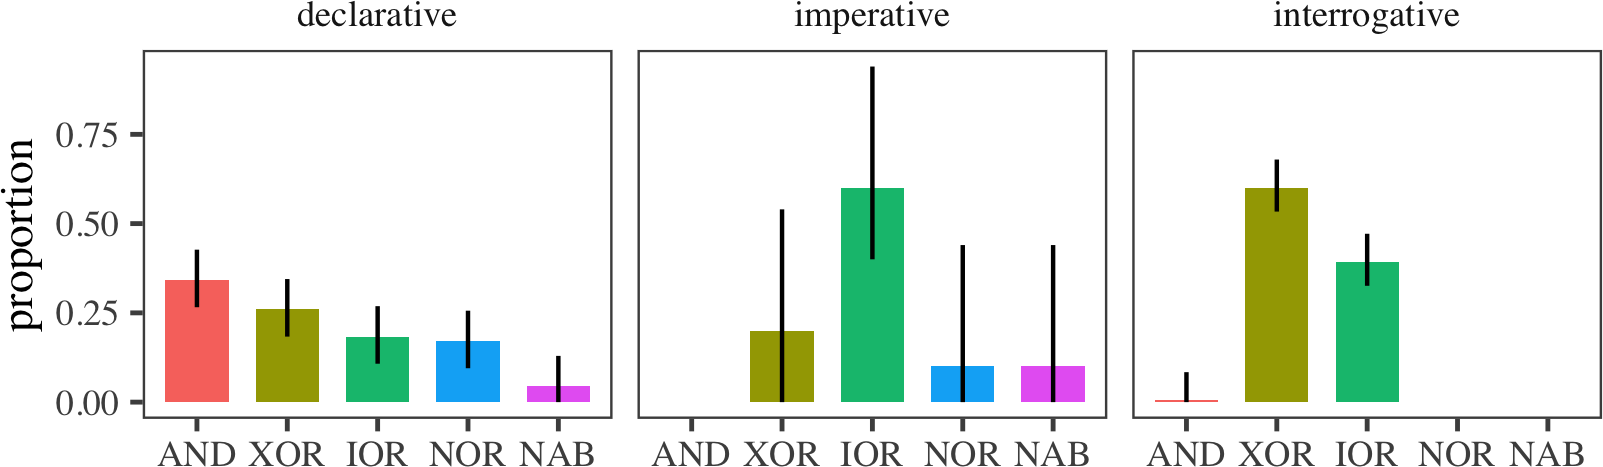
\includegraphics{figs/utterancePlot-1} 

}

\caption{Interpretations of disjunction with consistent disjuncts in interrogative, imperative, and declarative utterances.}\label{fig:utterancePlot}
\end{figure}

Next we we set aside cases with inconsistent disjuncts and look at instances of disjunction with consistent disjuncts. Figure \ref{fig:utterancePlot} shows their interpretations in declarative (N=158 utterances), interrogative (N=178 utterances), and imperative sentences (N=10 utterances). Interrogatives selected for either exclusive or inclusive interpretations. Imperatives were more likely to be interpreted as inclusive (IOR), but declaratives could receive almost any interpretation: conjunctive (AND), exclusive (XOR), inclusive (IOR), or even that ``neither'' disjunct was true (NOR). A common example of inclusive imperatives was invitation to action such as ``Have some food or drink!''. Such invitational imperatives seem to convey inclusivity (IOR) systematically, and often give the addressee full permission with respect to both alternatives. In fact, it can be odd to use them to imply exclusivity (e.g.~``Have some food or drink, but not both!''), and they are not conjunctive either; they do not invite the addressee to do both actions (e.g.~``Have some food, and have some drink!'').

\begin{figure}[H]

{\centering 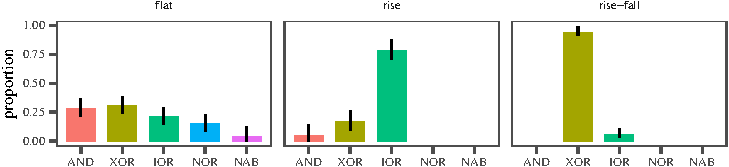
\includegraphics{figs/intonationPlot-1} 

}

\caption{Interpretations of disjunction with consistent disjuncts with flat, rising, or rise-fall intonation types.}\label{fig:intonationPlot}
\end{figure}

While interrogatives select for both exclusive and inclusive interpretations, their intonation can distinguish between the two. Figure \ref{fig:intonationPlot} shows the different intonation contours -- flat (N=186 utterances), rise (N=77 utterances), rise-fall (N=101 utterances) -- for the three interpretations of consistent disjunction. The rise and rise-fall contours are typical of interrogatives, and disjunctions with rise-fall contours are typically exclusive (XOR). With rising intonation, disjunctions are typically inclusive (IOR), and disjunctions with flat intonation could be exclusive (XOR), conjunctive (AND), inclusive (IOR), or neither (NOR). These results are consistent with Pruitt and Roelofsen (2013)'s experimental findings with adults on the role of intonation in the interpretation polar and alternative questions.

\begin{figure}[H]

{\centering 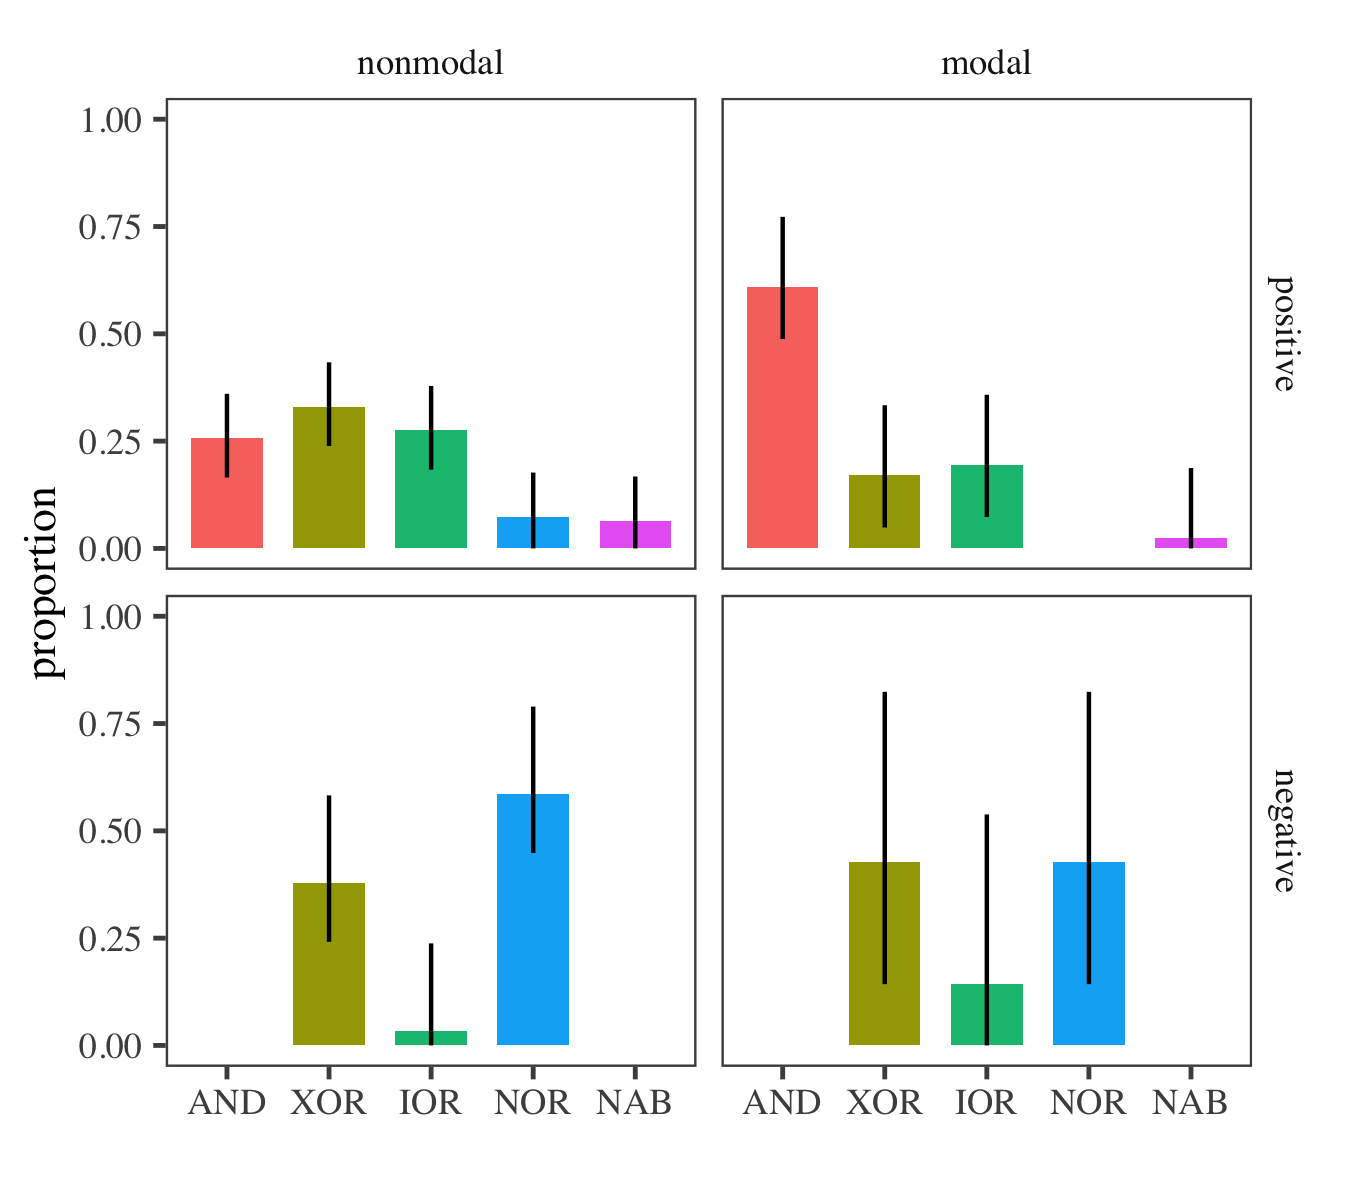
\includegraphics{figs/negModalPlot-1} 

}

\caption{Distribution of connective interpretations for consistent disjuncts with flat intonation broken down by whether a modal or negative morpheme was present in the utterance.}\label{fig:negModalPlot}
\end{figure}

What about consistent disjunctions with flat intonation? Figure \ref{fig:negModalPlot} presents the interpretations based on whether the utterance contained a negation or a modal (positive modal = 41, positive nonmodal = 109, negative modal = 7, negative nonmodal= 29). Disjunctions containing a modal like \emph{can} or \emph{maybe} were more likely to have a conjunctive interpretation. This is consistent with free-choice inferences (Kamp, 1973), where statements like ``you can have tea or coffee'' are interpreted conjunctively as ``you can have tea \emph{and} you can have coffee''. When the utterance contained a negation, the disjunction could be interpreted as exclusive (XOR) or as neither (NOR). These two interpretations correspond to the scope relations between negation and disjunction. If negation scopes above disjunction, we get a neither (NOR) interpretation (e.g.~``I do not eat cauliflower, cabbage or baked beans.''). But if disjunction scopes above negation, the interpretation is likely to be exclusive (e.g.~don't throw it at the camera or you're going in the house.) These results also suggest that learners who track the co-occurences of \emph{or} with negative morphemes can learn about the scope interaction of disjunction and negative particles in their native language.

\begin{figure}[H]

{\centering 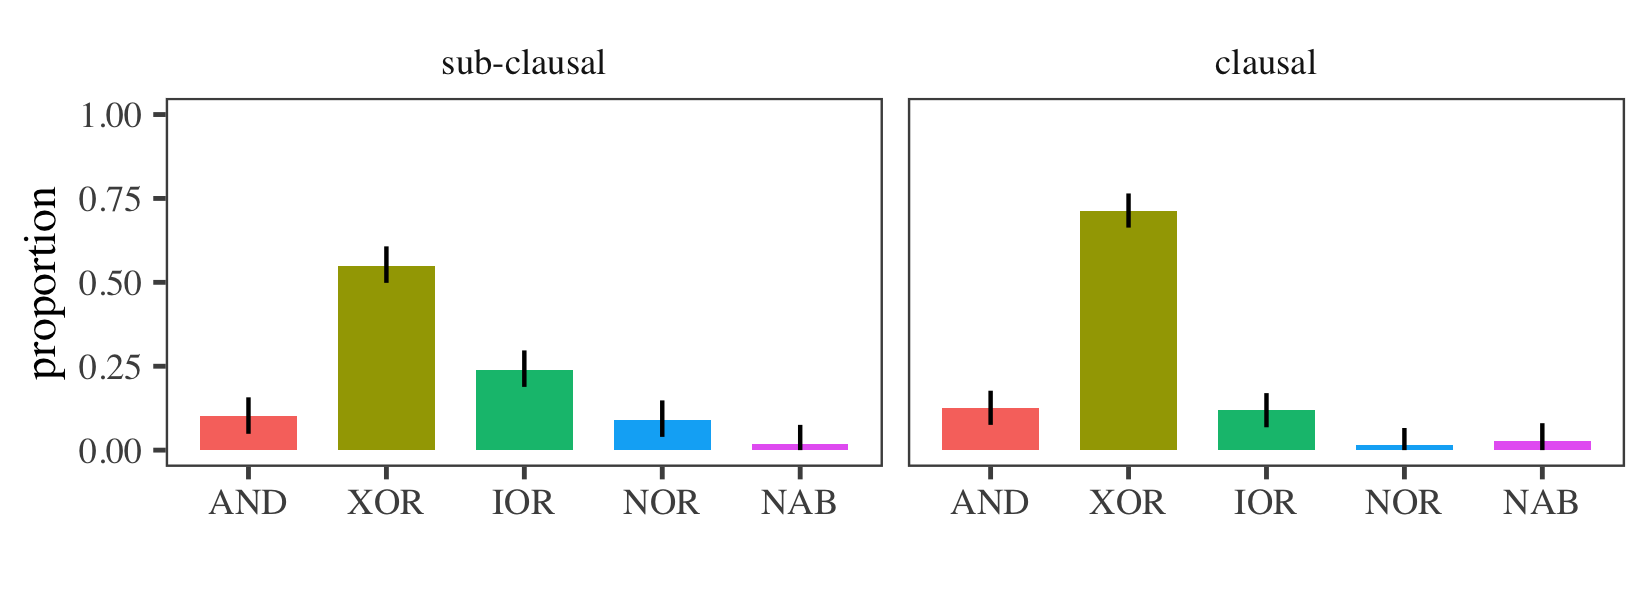
\includegraphics{figs/syntaxPlot-1} 

}

\caption{Interpretations of clausal vs. sub-clausal disjunction in all the annotated utterances.}\label{fig:syntaxPlot}
\end{figure}

The connective interpretations of the remaining two categories, syntactic level and communicative intent, are shown in Figures \ref{fig:syntaxPlot} and \ref{fig:speechActPlot}. For these categories, we show connective interpretations over all instances of disjunction. Figure \ref{fig:syntaxPlot} shows connective interpretations by syntactic level (sub-clausal = 329 utterances, clausal = 279 utterances). Over all annotated instances, disjunctions were more likely to be interpreted as exclusive if their disjuncts were clauses or verbs rather than nominals, adjectives, or prepositions (all sub-clausal units). As we noted earlier, the intuition here is that utterances like ``They had tea or coffee'' are less likely to be exclusive than ``they had tea or they had coffee.'' But syntactic level can be correlated with other factors predicting connective interpretation. As we will see in Study 3, a computational learning model did not find syntactic level useful in classifying instances of disjunction, compared to other annotation categories.

\begin{figure}[H]

{\centering 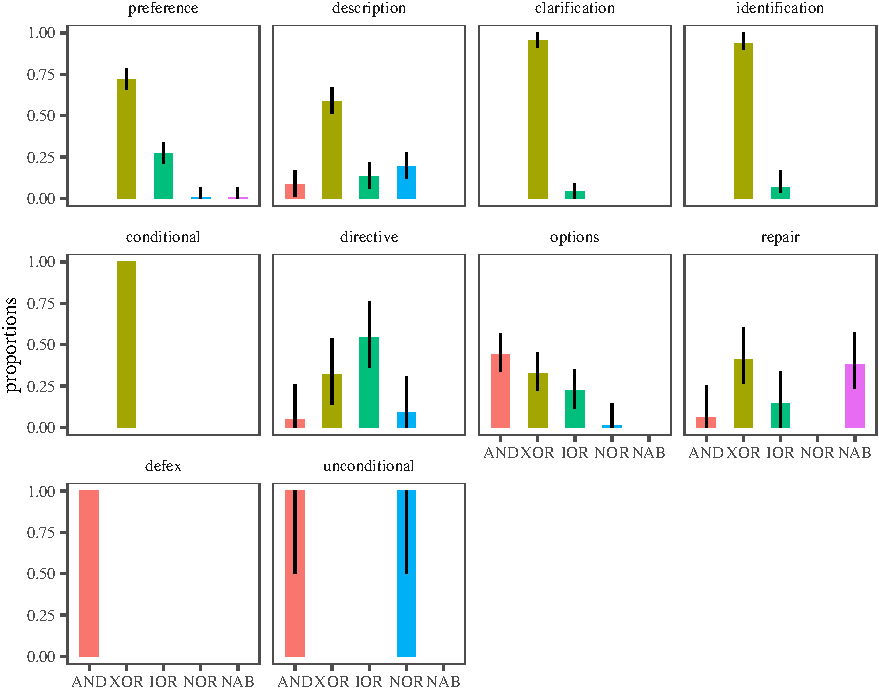
\includegraphics{figs/speechActPlot-1} 

}

\caption{Interpretations of disjunction in different communicative functions.}\label{fig:speechActPlot}
\end{figure}

Figure \ref{fig:speechActPlot} shows the connective interpretations for the 10 different communicative functions annotated here (Number of utterances: clarification = 45, conditional = 32, definitions and examples = 17, description = 150, directive = 22, identification = 30, options = 77, preference = 199, repair = 34, unconditional = 2). With certain functions, the likelihood of some interpretations was higher. An exclusive interpretation (XOR) was common in acts of clarification, identification, stating/asking preferences, stating/asking about a description, or making a conditional statements. These results are consistent with expectations about the communicative intentions these kinds of speech acts carry. In clarifications, the speaker needs to know which of two alternatives the other party intended. In identifications, the speaker needs to know which category a referent belongs to. In preferences, the parent seeks to know which alternative the child wants. Even though descriptions can be either inclusive or exclusive, in the current sample most descriptions were questions about the state of affairs and required the child to provide one of the alternatives as the answer. In conditionals such as ``come here or you are grounded'', the point of the threat was that only one disjunct could be true: either ``you come and you are not grounded'' or ``you don't come and you are grounded''.

Repairs often received an exclusive (XOR) or a second-disjunct-true (NAB) interpretation. This is predictable given that in making a repair, the speaker intends to say that the first disjunct is inaccurate or incorrect. Unconditionals and definitions/examples always had a conjunctive interpretation (AND). Again, this is predictable: the speaker intends to communicate that all options apply. If the mother says that ``cats are animals like lions or tigers'', she intends to say that both lions and tigers are cats, and not one or the other. Interestingly, in some cases, \emph{or} can even be replaced by \emph{and}: ``cats are animals like lions and tigers''. In unconditionals, the speaker communicates that, for both alternatives, a certain proposition holds. For example, if the mother says ``ready or not, here I come!'', she communicates that ``I come'' is true both when the child is ready and when the child is not ready.

The category ``options'' contained examples of free-choice inferences such as ``you could drink orange juice or apple juice''. These were often interpreted as conjunctive (AND) or as inclusive (IOR). We found that free-choice utterances were more common in child-directed speech than previously assumed. Finally, directives received either an IOR or XOR interpretation. Note that the most common communicative functions in our sample were preferences and descriptions. Other communicative functions such as unconditionals or options were fairly rare. But despite their rarity, such constructions must eventually be learned by children since almost all adults know how to interpret them.

\hypertarget{conclusion}{%
\subsection{Conclusion}\label{conclusion}}

This study focused on the interpretations that connectives \emph{and} and \emph{or} received in child-directed speech. It also investigated certain cues that appear to help children in their learning of these interpretations. We annotated examples of \emph{and} and \emph{or} in child-directed speech for their truth-conditional interpretations, along with six candidate cues to interpretation: logical consistency, utterance type, intonation, negative or modal morphemes, syntactic level of the coordinands, and the communicative function of the utterance. Like Morris (2008), we found that the most common interpretations of \emph{and} and \emph{or} are conjunction (AND) and exclusive disjunction (XOR) respectively. So if children relied only on the presence of connective word forms, they should assign \emph{and} the meaning of conjunction and \emph{or} the meaning of exclusive disjunction.

But we also found that the most likely interpretation of a disjunction depended on the cues that co-occurred with it in context. A disjunction was most likely exclusive if the alternatives were inconsistent (i.e.~contradictory). If the alternatives were consistent, then the disjunction could be either inclusive or exclusive. In questions, if the intonation on the disjunction was rising, it was inclusive, and if the intonation was rise-fall, it was mostly likely exclusive. In declaratives and imperatives with flat intonation, disjunctions were most likely interpreted as AND if there was a modal present, and as NOR or XOR if there was a negation present in the utterance. Finally, in the absence of any of these cues, a disjunction was more likely to be non-exclusive (IOR + AND) than exclusive (XOR). Several cues therefore can carry informational value about the interpretation of disjunction, and learners can make use of these to arrive at the relevant interpretation in context. While this is a reasonable conjecture from the pattern of data in our annotation study, we have not yet presented any formal model or statistical analysis that can determine the relative utility of these cues in predicting connective interpretations. Given that we have several predictors that might be correlated and we want to select for a parsimonious set of explanatory predictors, we use decision tree learning (instead of linear regression) in Study 3 to implement and test our cue-based model of learning connective interpretations.

\hypertarget{study-3-the-computational-model}{%
\section{Study 3: The Computational Model}\label{study-3-the-computational-model}}

In this study, we use a computational learning model to formalize the context-dependent account of learning linguistic disjunction. Our computational model represents an ideal observer (Geisler, 2003) who has access to data labeled for the cues discussed in Study 2 as well as the interpretation of a disjunction. The task of the model is to learn to use the available cues to predict the interpretation of a new disjunction. Such a model provides two major contributions. First, it provides ``proof of concept'' for the context-dependent account presented in the paper, showing that it is possible to learn the interpretation of a disjunction using the cues in Study 2. Second, it can help us quantify and understand how useful each cue is to the learner, by systematically selecting and ordering cues that have higher informational value for the interpretation of disjunction.

A decision tree is a classification model structured as a hierarchical tree with an initial node, called the root, that branches into more nodes until it reaches the leaves (Breiman, 2017). Each node represents a test on a feature, each branch represents an outcome of the test, and each leaf represents a classification label. With a decision tree, observations can be classified or labeled based on a set of features.

Decision trees have at least four advantages for modeling cue-based accounts of semantic acquisition. First, the features used in decision trees for classification can stand for the cues that help in the acquisition and interpretation of a word or an utterance. Second, the degree to which a decision tree relies on available cues in the data can be varied, and so test cue-based models to varying degrees. Third, unlike many other machine learning techniques, decision trees result in models that are interpretable. Fourth, the order of decisions or features used for classification is based on information gain. Features that appear higher (earlier) in the tree are more informative and helpful for classification. Decision trees, therefore, can help us understand which cues are more helpful for semantic acquisition.

Decision tree learning is the construction of a decision tree from labeled training data. We applied decision tree learning to the annotated data of Study 2 by constructing random forests (Breiman, 2001; Ho, 1995). In random forest classification, multiple decision trees are constructed on subsets of the data, and each tree predicts a classification. The ultimate outcome is a majority vote of each tree's classification. Since decision trees tend to overfit data, random forests control for overfitting by building more trees and averaging their results (Breiman, 2001; Ho, 1995).

\hypertarget{methods-2}{%
\subsection{Methods}\label{methods-2}}

The random forest models were constructed using python's Sci-kit Learn package (Pedregosa et al., 2011). The annotated data had a feature array and a connective interpretation label for each connective use. Connective interpretations included exclusive (XOR), inclusive (IOR), conjunctive (AND), neither (NOR), and NAB which states that only the second proposition is true. The features or cues used included the following annotation categories: intonation, consistency, utterance type, syntactic level, negation, and communicative function. All models were trained with stratified 10-Fold cross-validation to reduce overfitting. Stratified cross-validation maintains the distribution of the initial data in the random sampling to build cross-validated models. Maintaining the data distribution ensures a more realistic learning environment for the forests. Tree success was measured with F1-Score, harmonic average of precision and recall (Rijsbergen, 1979).

We first ran a grid search on the hyperparameter space to establish the number of trees in each forest and the maximum tree depth allowable. The grid search creates a grid of all combinations of forest size and tree depth and then trains each forest from this grid on the data. The forests with the best F1-score and lowest size/depth are reported (Pedregosa et al., 2011). The default number of trees for the forests was set to 20, with a max depth of eight and a minimum impurity decrease of zero. Impurity was measured with Gini impurity, which states the odds that a random member of the subset would be mislabled if it were randomly labeled according to the distribution of labels in the subset (Gini, 1912).

Decision trees were fit with high and low minimum-Gini-decrease values. High minimum-Gini-decrease results in a tree that does not use any features for branching. Such a tree represents the baseline or traditional approach to mapping that maps a word directly to its most likely interpretation. Low minimum-Gini-decrease allows for a less conservative tree that uses multiple cues or features to predict the interpretation of a disjunction. Such a tree represents the cue-based context-sensitive account of word learning.

\hypertarget{results-1}{%
\subsection{Results}\label{results-1}}

We first present the results of the random forests in a binary classification task where the models were trained to classify whether an interpretation was exclusive or not. In the next section, we use a more general classifier to predict all interpretations of disjunction using the annotated cues. For visualization of trees, we selected the highest performing tree in the forest by testing each tree and selecting for highest F1 score. While the forest's performance is not identical to the highest performing tree, the best tree illustrates successful learning from data.

\hypertarget{detecting-exclusivity}{%
\subsubsection{Detecting Exclusivity}\label{detecting-exclusivity}}

Figure \ref{fig:binaryFigure}A shows the best performing decision tree with high minimum Gini decrease. As expected, a learner that does not use any cues would interpret \emph{or} as exclusive all the time. This is the baseline model. Figure \ref{fig:binaryFigure}B shows the best performing decision tree with low minimum Gini decrease. The tree has learned to use intonation and consistency to classify disjunctions as exclusive or inclusive. As expected, if the intonation is rise-fall or the disjuncts are inconsistent, the interpretation is exclusive. Otherwise, the disjunction is classified as not exclusive.

Figure \ref{fig:binaryFigure}C shows the average F1 scores of the baseline and cue-based models in classifying exclusive examples as the number of training examples increases. The models perform similarly, but the cue-based model performs slightly better. The real difference between the baseline model and the cue-based model is in their performance on inclusive examples. Figure \ref{fig:binaryFigure}D shows the F1 score of the forests as a function of the training size in classifying inclusive examples. As expected, the baseline model performs poorly while the cue-based model improves with more examples and performs better than the baseline tree.

\begin{figure}
\centering
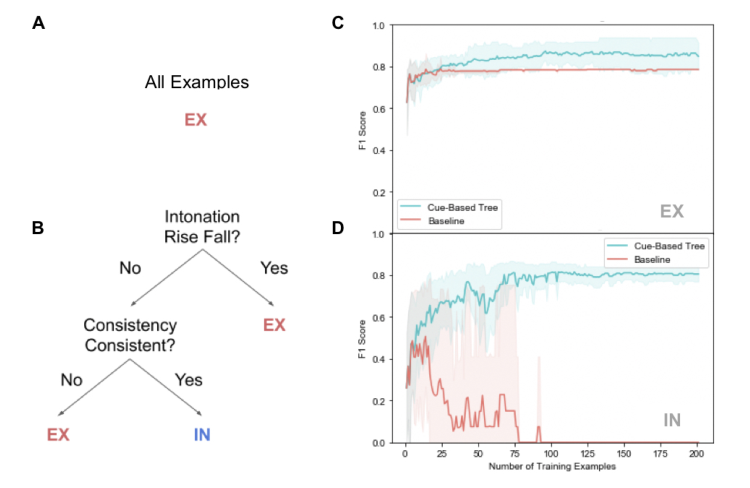
\includegraphics{figs/binaryFigure-1.pdf}
\caption{\label{fig:binaryFigure}(A) The structure for the baseline (highest Gini threshold, 0.2) decision tree trained on examples with exclusive (EX) and non-exclusive (IN) interpretations. (B) The structure for the cue-based decision tree (low Gini threshold of 0.01). The average F1 score with 95\% confidence intervals as a function of the number of training examples in the baseline and cue-based model when treating as positive (C) EX and (D) IN respectively.}
\end{figure}

\hypertarget{detecting-all-interpretations}{%
\subsubsection{Detecting All Interpretations}\label{detecting-all-interpretations}}

We next look at decision trees trained on the annotation data to predict all the interpretation classes for disjunction: AND, XOR, IOR, NOR, and NAB. Figure \ref{fig:wholeFigure}A shows the baseline model that only uses the words \emph{and} and \emph{or} to classify. As expected, \emph{and} receives a conjunctive interpretation (AND) and \emph{or} receives an exclusive interpretation (XOR). Figure \ref{fig:wholeFigure}B shows the best example tree of the cue-based model. The leaves of the tree show that it recognizes exclusive, inclusive, conjunctive, and even neither (NOR) interpretations of disjunction. How does the tree achieve that? Like the baseline model, the tree first asks about the connective used: \emph{and} vs.~\emph{or}. Then like the previous cue-based model, it asks about intonation and consistency. If the intonation is rise-fall, or the disjuncts are inconsistent, the interpretation is exclusive. Then it asks whether the sentence is an interrogative or a declarative. If interrogative, it guesses an inclusive interpretation. This basically covers questions with a rising intonation. Then the tree picks declarative examples that have conditional speech act (e.g.~``give me the toy or you're grounded'') and labels them as exclusive. Finally, if negation is present in the sentence, the tree labels the disjunction as NOR.

Figures \ref{fig:wholeFigure}C, \ref{fig:wholeFigure}D, and \ref{fig:wholeFigure}E show the average F1-scores for the conjunctive (AND), exclusive (XOR), and inclusive (IOR) interpretations as a function of training size. While the cue-based model generally performs better than the baseline model, it shows substantial improvement in classifying inclusive cases. Figure \ref{fig:wholeFigure}F shows the average F1-score for the neither interpretation as a function of training size. Compared to the baseline model, the cue-based model shows a substantially better performance in classifying negative sentences. The success of the model in classifying neither examples (NOR) suggests that the cue-based model offers a promising approach for capturing the scope relation of operators such as negation and disjunction. Here, the model learns that when negation and disjunction are present, the sentence receives a neither (NOR) interpretation. In other words, the model has learned the narrow-scope interpretation of negation and disjunction from the input data. In a language where negation and disjunction receive an XOR interpretation (not A or not B), the cue-based model can learn the wide-scope interpretation of disjunction.

Finally, Figure \ref{fig:wholeFigure}G shows the average F1 score for the class NAB. This disjunct interpretation suggested that the first disjunct is false but the second true. NAB was by-far the most infrequent of the considered disjuncts (n=6), was not in every tree in the random forests, and was not present in the highest performing tree. However, considering the data, it was seen in examples of repair most often and the most likely cue to it was also the communicative function or speech act of repair. The results show that even though there were improvements in the cue-based model, they were not stable as shown by the large confidence intervals. It is possible that with larger training samples, the cue-based model can reliably classify the NAB interpretations as well.

\begin{figure}
\centering
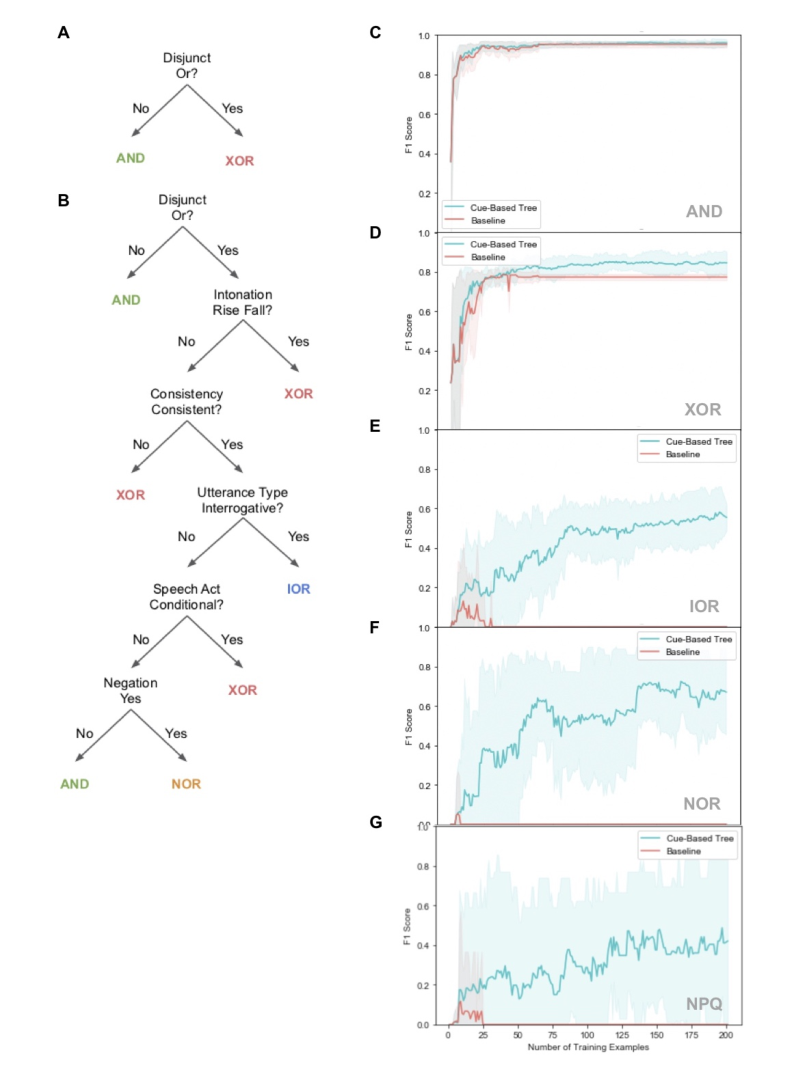
\includegraphics{figs/wholeFigure-1.pdf}
\caption{\label{fig:wholeFigure}(A) The structure for the baseline (highest Gini threshold, 0.2) decision tree trained on examples with XOR, IOR, AND, and NOR interpretations. (B) The structure for the cue-based decision tree (low Gini threshold of 0.01). The average F1 score with 95\% confidence intervals as a function of the number of training examples in the baseline and cue-based model when treating as positive (C) AND, (D) XOR, (E) IOR, (F) NOR respectively.}
\end{figure}

\hypertarget{conclusion-1}{%
\subsection{Conclusion}\label{conclusion-1}}

In this study, we used the annotation data from Study 2 to train and compare two random forest models representing two theoretical accounts of the acquisition of disjunction. The first account was a baseline (context-independent) account in which words are isolated and directly mapped to their most likely meanings, disregarding available contextual cues. Random forest models with high minimum-Gini-impurity-decrease represented this account. The second account was what we called the cue-based context-dependent mapping in which words are mapped to meanings using a set of cues available in the context. Random forest models with low minimum-Gini-impurity-decrease represented this cue-based account. Comparison of the F1-Scores produced by models representing these two accounts showed that the cue-based models outperformed the baseline models in every classification task. Most importantly, while the baseline models learned to always interpret a disjunction as exclusive, the cue-based models learned to interpret a disjunction as exclusive, inclusive, conjunctive, or neither (NOR), depending on the cues available in the input.

\hypertarget{general-discussion}{%
\section{General Discussion}\label{general-discussion}}

We have presented three studies to support the claim that child-directed speech contains linguistic cues for the successful interpretation of linguistic disjunction, and that mapping \emph{or} to its meaning in a cue-based context-dependent manner addresses ``the puzzle of learning disjunction''. Study 1 presented the overall distribution of \emph{or} and \emph{and} in parents' and children's speech in CHILDES corpora. It showed that children heard 1-2 instances of \emph{or} per 1000 words produced by parents. Children started producing \emph{or} themselves between 18-30 months, and by 42 months attained a rate of one \emph{or} per 1000 words. Study 2 showed that, as Morris (2008) had also shown, the most common interpretation of \emph{or} in child-directed speech was exclusive disjunction. These exclusive interpretations were accompanied by prosodic and semantic cues. In the absence of these cues to exclusivity, the interpretation of a disjunction was most likely non-exclusive. Finally, Study 3 used decision-tree learning to show that an ideal learner can use these linguistic cues to partition the input and predict the intended interpretation of a linguistic disjunction.

Here we address some important limitations of the present account that future work should address. The computational model in study 3 represents an ideal observer (Geisler, 2003). It allows us measure the information available in the input for mapping \emph{or}, provides a computational account of how to perform this task, and serves as a starting point for developing more realistic models. Future research should aim to improve at least three important aspects of this model. First, the model had access to a limited set of pre-selected cues for learning. As in other cue-based accounts (Monaghan \& Christiansen, 2014), this account needs to explain how the learner discovers and selects which cues are relevant to the acquisition of disjunction, among potentially many possible candidate cues. Fortunately the cues relevant for the acquisition of \emph{or} are not idiosyncratic. Intonation and the semantics of the neighboring words are cues that need to be monitored for the interpretation of almost any word. It is therefore possible that a limited number of salient cues in child-directed speech guide many form-meaning mappings, and future research will uncover these.

Second, our account and computational model assumed the 16 binary logical connective concepts for the mapping of \emph{or}. Future research on this account, as well as on other accounts of learning disjunction, needs to explain how children limit their conceptual space to consider only connective concepts when mapping words like \emph{and} and \emph{or}. One approach that may contribute to this is syntactic bootstrapping (Brown, 1957; Gleitman, 1990). Previous research has shown that syntactic bootstrapping can help learners filter their conceptual space appropriately for many word classes such as nouns (Soja, 1992), verbs (Naigles, 1990), adjectives (Taylor \& Gelman, 1988), and prepositions (Landau \& Stecker, 1990). It seems probable that a similar mechanism applies to connectives, especially that coordination has specific syntactic properties crosslinguistically (see Haspelmath, 2007). Coordinators combine two or more units of the same type and return a larger unit, also of the same type. This larger unit bears the same semantic relation to the surrounding words, as the smaller units did without the coordination. These properties distinguish coordinators from other function words.

Third, the ideal observer/learner model was implemented using a supervised learning algorithm and had access to labeled training data. While it is not clear what feedback children receive while learning function words like \emph{or}, it is clear that they do not have access to the kind of labeled data in our model. Future work should revise this aspect of the model and incorporate the kinds of feedback children actually receive (Chouinard \& Clark, 2003; Clark, 2010).

Fourth, this research has demonstrated the utility of cues for the acquisition of disjunction, but future experimental work needs to show that children are indeed sensitive to such cues and in fact use them in the acquisition of \emph{or}. Some research, for example, already suggests that infants are sensitive to intonational cues. Frota, Butler, and Vigário (2014) have shown that 5-9 month-olds discriminate rising yes/no intonation typical for questions from the falling intonation typical for assertions. And Esteve-Gibert, Prieto, and Liszkowski (2017) showed that 12 month-olds can use gesture and intonation to distinguish basic speech acts like commands and statements. Such findings suggest that by the time children start their early mappings for disjunction, they may already be sensitive to the role of intonation in conveying some aspects of linguistic meaning. However, whether they actually use such cues to learn the meaning of function words like \emph{or} remains an open question.

Fifth, our findings do not speak against specific theoretical accounts regarding the semantic and pragmatic status of disjunctive interpretations. In formal semantics and pragmatics, it is common to assume that the primary meaning of \emph{or} is inclusive disjunction. The exclusive interpretation is derived using secondary enhancements to this primary meaning, for example by Gricean reasoning about the alternative connective \emph{and}, which results in an exclusivity implicature Chierchia et al. (2004). Such accounts can accommodate our findings by assuming that different cues discussed in this paper are related to specific semantic and pragmatic mechanisms that deliver the intended connective interpretation. For example, a rise-fall intonation may underlyingly cue a mechanism that strengthens the basic inclusive semantics of \emph{or} into exclusive disjunction (see Roelofsen \& Gool, 2010 for a formal treatment of disjunction and intonation along these lines). Similarly, when the individual disjuncts are inconsistent (e.g.~clean or dirty) the learner can derive an exclusive interpretation using the composition of exclusive disjuncts and an inclusive meaning for \emph{or}. Such accounts have to then explain how the learner maps the cues to the correct underlying mechanism. Alternatively, it is possible to assume no underlying mechanism and directly map the cues along with the connective word \emph{or} to the intended interpretation. These cues can later help disambiguate a disjunction in a specific context. Such an account would be closer to the usage-based tradition of language acquisition and processing (Goldberg, 2003; Langacker, 1987; Tomasello, 2003). The challenge for such accounts is to explain the universal tendencies in disjunctive interpretations and the mechanisms that generate them. Therefore, different theoretical accounts of disjunction can accommodate the findings of this paper and provide more specific predictions for future research.

Finally, this research should be placed within the larger context of word learning. As we noted earlier, Quine (1960) proposed three strategies for lexical learning: isolated mapping, context-dependent mapping, and description mapping. First, children learn many content words -- concrete nouns, adjectives, and verbs -- by mapping their isolated forms to concepts that are created through sensory experience. For example, a child may associate \emph{dirty} with a visible property of objects or \emph{sit} with the action she performs before having food or wearing shoes. Second, for more abstract meanings like those of some function words, children also rely on the meanings of the surrounding concrete content words on the utterance. For example, hearing ``sit and eat'' or ``clean and shiny'' may allow children to infer that the connective \emph{and} is used when the speaker intends both actions or properties. Connective \emph{or}, on the other hand, appears commonly in constructions like ``sit or stand'' and ``clean or dirty'' where only one or the other action or property can apply in typical everyday contexts. Third, once children have learned enough isolated and context-dependent mappings of meanings, they can also make use of linguistic definitions. For example, children may learn from their parents that \emph{below} is ``another word for under'' or that \emph{carving} is ``cutting wood'' (see Clark, 2010). Gleitman et al. (2005)'s ``syntactic bootstrapping'' offers a similar developmental account with emphasis on the role of syntactic structure in learning the meaning of ``hard words'' like mental verbs (e.g., \emph{think} and \emph{know}). They argue for a general probabilistic learning mechanism that combines and coordinates multiple cues such as the number of the verb's arguments, the argument position (subject vs.~object), as well as argument type (the type of meanings the arguments have) to constrain the hypothesis space for verb meanings.

Our account of English disjunction presented here is in line with both Quine (1960) and Gleitman et al. (2005), and contributes to word meaning mapping in at least four respects. First, we have highlighted the role of prosody in the mapping of meaning. Prosody is considered an important source of information for learning a language's structure (Carvalho, He, Lidz, \& Christophe, 2019) and our work suggests that it can also play an important role in addressing the form-meaning mapping problem. Second, we have emphasized the role of semantic relations among known words in an utterance as a cue in mapping meanings; something Gleitman et al. (2005) discuss under the label of ``distributional cues''. The present work on disjunction also shows that the entailment relations between disjuncts, and more specifically whether they lead to logical inconsistency, can help learners map the meaning of a disjunctive term like \emph{or}. Third, our findings show that cues may play a more complex role than previously assumed. Previous literature has shown that cues can boost a particular hypothesis against another to reduce uncertainty. Our work suggests that cues may also affect the mapping mechanism itself. With respect to disjunction, cues can break down the input into each ``context of use'' and allow the learner to map words to their meanings in a context-dependent manner. Fourth, in using decision-tree learning, our account takes some initial steps toward quantifying and formalizing the probabilistic cue-integration, as advocated by Gleitman et al. (2005). Ultimately, we need to discover further cues and mechanisms that aid the acquisition of abstract functional meanings, and so establish a more comprehensive theory of word learning in first language acquisition.

\hypertarget{appendix}{%
\section{Appendix}\label{appendix}}

Figure \ref{fig:oReliabilityPlot} shows the percentage agreement and the kappa values for each annotation category over the 8 iterations.

\begin{figure}[H]

{\centering 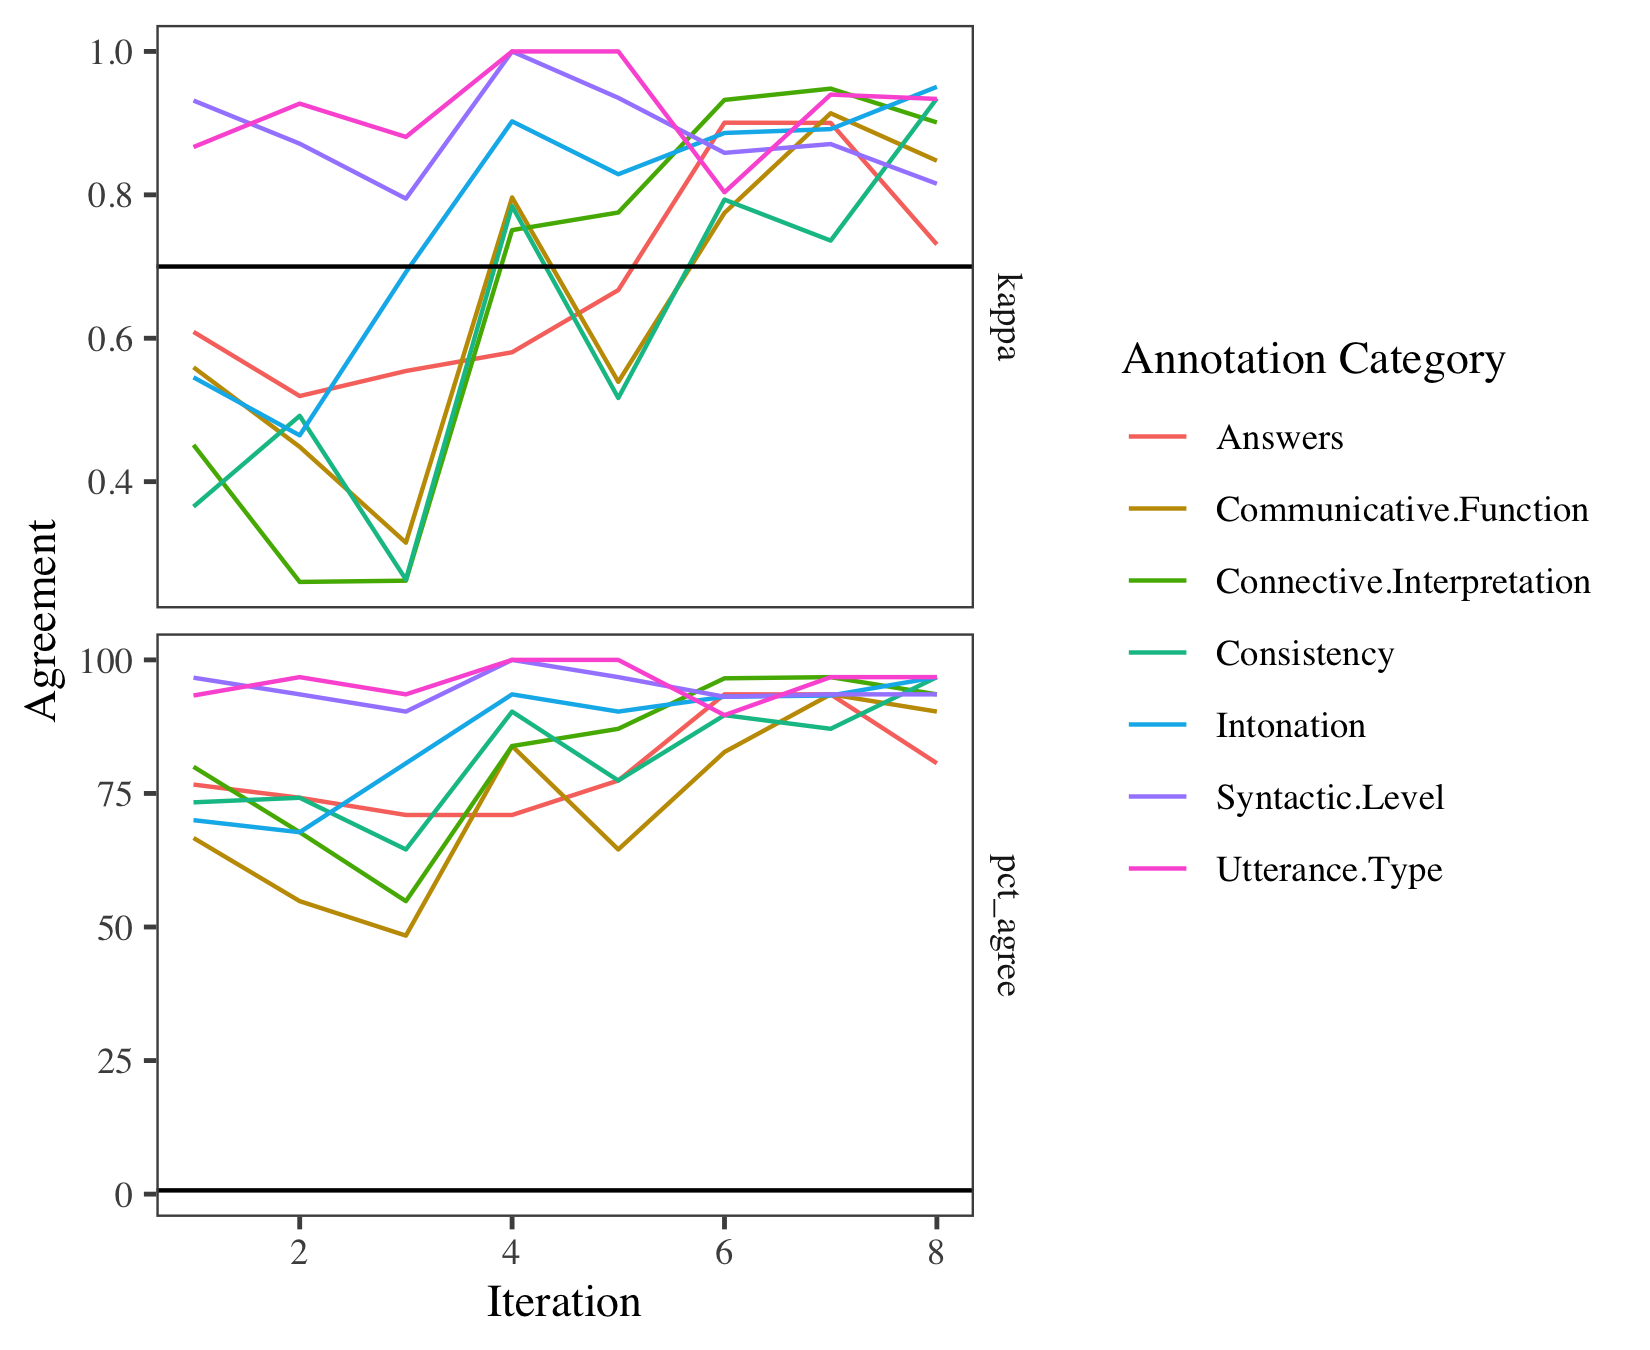
\includegraphics{figs/oReliabilityPlot-1} 

}

\caption{Inter-annotator agreement for disjunction examples.}\label{fig:oReliabilityPlot}
\end{figure}

Agreement in the following three categories showed substantial improvement after better and more precise definitions and annotation criteria were developed: connective interpretation, intonation, and communicative function. First, connective interpretation showed major improvements after annotators developed more precise criteria for selecting the propositions under discussion and separately wrote down the two propositions connected by the connective word. For example, if the original utterance was ``do you want milk or juice?'', the annotators wrote ``you want milk, you want juice'' as the two propositions under discussion. This exercise clarified the exact propositions under discussion and sharpened annotator intuitions with respect to the connective interpretation that is communicated by the utterance. Second, annotators improved agreement on intonation by reconstructing an utterance's intonation for all three intonation categories. For example, the annotator would examine the same sentence ``do you want coffee or tea?'' with a rise-fall, a rise, and a flat intonation. Then the annotator would listen to the actual utterance and see which one most resembled the actual utterance. This method helped annotators judge the intonation of an utterance more accurately. Finally, agreement on communicative functions improved as the definitions were made more precise. For example, the definition of ``directives'' in Table \ref{tab:speechActs} explicitly mentions the difference between ``directives'' and ``options''. Clarifying the definitions of communicative functions helped improve annotator agreement.

Inter-annotator reliability for conjunction was calculated in the same way. Two different annotators coded 300 utterances of \emph{and}. Inter-annotator reliability was calculated over 10 iterations of 30 examples. Figure \ref{fig:andReliabilityPlot} shows the percentage agreement between the annotators as well as the kappa values for each iteration. Despite high percentage agreement between annotators, the kappa values did not pass the set threshold of 0.7 in three consecutive iterations. This paradoxical result is mainly due to a property of kappa. An imbalance in the prevalence of annotation categories can drastically lower its value. When one category is extremely common with high agreement while other categories are rare, kappa will be low (Cicchetti \& Feinstein, 1990; Feinstein \& Cicchetti, 1990). In almost all annotated categories for conjunction, there was one class that was extremely prevalent. In such cases, it is more informative to look at the class specific agreement for the prevalent category than the overall agreement measured by Kappa (Cicchetti \& Feinstein, 1990; Feinstein \& Cicchetti, 1990).

\begin{figure}[H]

{\centering 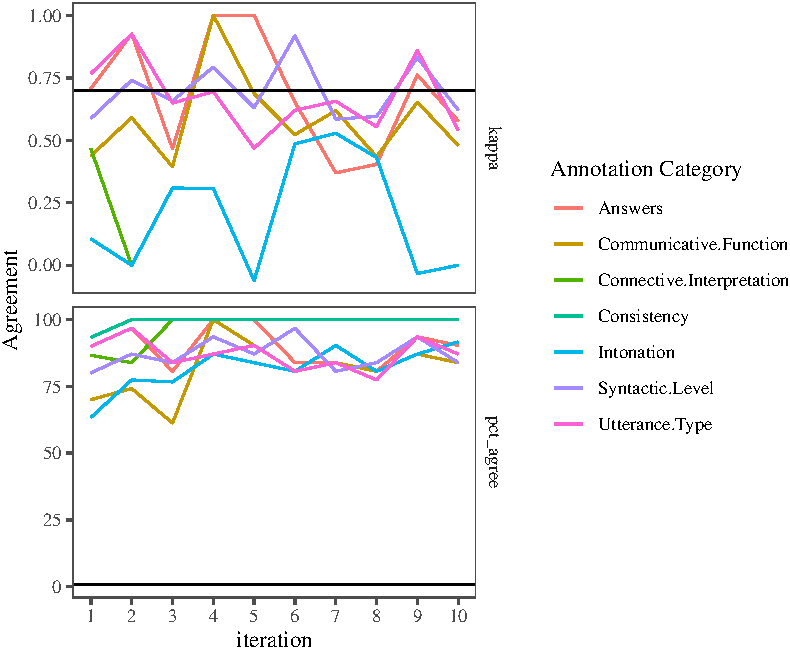
\includegraphics{figs/andReliabilityPlot-1} 

}

\caption{Inter-annotator agreement for conjunction examples.}\label{fig:andReliabilityPlot}
\end{figure}

Table \ref{tab:andAgreeStats} lists the dominant classes as well as their prevalence, the values of class specific agreement index, and category agreement index (Kappa). Class specific agreement index is defined as \(2n_{ii}/n_{i.}+n_{.i}\), where \(i\) represents the class's row/column number in the category's confusion matrix, \(n\) the number of annotations in a cell, and the dot ranges over all the row/column numbers (Fleiss, Levin, \& Paik, 2013, p. 600; Ubersax, 2009). The class specific agreement indices are high for all the most prevalent classes showing that the annotators had very high agreement on these class, even though the general agreement index (Kappa) was often low. The most extreme case is the category ``consistency'' where almost all instances were annotated as ``consistent'' with perfect class specific agreement but low overall Kappa. In the case of utterance type and syntactic level where the distribution of instances across classes was more even, the general index of agreement Kappa is also high. In general, examples of conjunction showed little variability across annotation categories and mostly fell into one class within each category. Annotators had high agreement for these dominant classes.

\begin{table}

\caption{\label{tab:andAgreeStats}Most prevalent annotation class in each annotation category with the values of class agreement indeces and category agreement indeces (Kappa).}
\centering
\begin{tabular}[t]{l|l|r|r|r}
\hline
Annotation Category & Class & Prevalence & Class Agreement Index & Kappa\\
\hline
intonation & flat & 0.86 & 0.89 & 0.24\\
\hline
interpretation & AND & 0.96 & 0.98 & 0.39\\
\hline
answer & NA & 0.84 & 0.94 & 0.67\\
\hline
utterance\_type & declarative & 0.76 & 0.94 & 0.70\\
\hline
communicative\_function & description & 0.77 & 0.90 & 0.59\\
\hline
syntactic\_level & clausal & 0.67 & 0.91 & 0.70\\
\hline
consistency & consistent & 0.99 & 1.00 & 0.50\\
\hline
\end{tabular}
\end{table}

\hypertarget{references}{%
\section{References}\label{references}}

\setlength{\parindent}{-0.5in}
\setlength{\leftskip}{0.5in}

\hypertarget{refs}{}
\begin{CSLReferences}{1}{0}
\leavevmode\vadjust pre{\hypertarget{ref-Aloni2016}{}}%
Aloni, M. (2016). Disjunction. In E. N. Zalta (Ed.), \emph{The {S}tanford encyclopedia of philosophy}. Stanford University. Retrieved from \url{https://plato.stanford.edu/archives/win2016/entries/disjunction/}

\leavevmode\vadjust pre{\hypertarget{ref-baldwin1993infants}{}}%
Baldwin, D. (1993). Infants' ability to consult the speaker for clues to word reference. \emph{Journal of Child Language}, \emph{20}(2), 395--418.

\leavevmode\vadjust pre{\hypertarget{ref-braine1981development}{}}%
Braine, M. D., \& Rumain, B. (1981). Development of comprehension of {``or''}: Evidence for a sequence of competencies. \emph{Journal of Experimental Child Psychology}, \emph{31}(1), 46--70.

\leavevmode\vadjust pre{\hypertarget{ref-breiman2001random}{}}%
Breiman, L. (2001). Random forests. \emph{Machine Learning}, \emph{45}(1), 5--32.

\leavevmode\vadjust pre{\hypertarget{ref-breiman2017classification}{}}%
Breiman, L. (2017). \emph{Classification and regression trees}. London: Routledge.

\leavevmode\vadjust pre{\hypertarget{ref-brown1957linguistic}{}}%
Brown, R. W. (1957). Linguistic determinism and the part of speech. \emph{The Journal of Abnormal and Social Psychology}, \emph{55}(1), 1.

\leavevmode\vadjust pre{\hypertarget{ref-cameron2003construction}{}}%
Cameron-Faulkner, T., Lieven, E., \& Tomasello, M. (2003). A construction based analysis of child directed speech. \emph{Cognitive Science}, \emph{27}(6), 843--873.

\leavevmode\vadjust pre{\hypertarget{ref-de2019prosody}{}}%
Carvalho, A. de, He, A. X., Lidz, J., \& Christophe, A. (2019). Prosody and function words cue the acquisition of word meanings in 18-month-old infants. \emph{Psychological Science}, \emph{30}(3), 319--332.

\leavevmode\vadjust pre{\hypertarget{ref-chierchia2004scalar}{}}%
Chierchia, G. et al. (2004). Scalar implicatures, polarity phenomena, and the syntax/pragmatics interface. \emph{Structures and Beyond}, \emph{3}, 39--103.

\leavevmode\vadjust pre{\hypertarget{ref-chierchia2001acquisition}{}}%
Chierchia, G., Crain, S., Guasti, M. T., Gualmini, A., \& Meroni, L. (2001). The acquisition of disjunction: Evidence for a grammatical view of scalar implicatures. \emph{Proceedings of the 25th {B}oston {U}niversity Conference on Language Development}, 157--168. Somerville, MA: Cascadilla Press.

\leavevmode\vadjust pre{\hypertarget{ref-chierchia2012grammatical}{}}%
Chierchia, G., Fox, D., \& Spector, B. (2012). The grammatical view of scalar implicatures and the relationship between semantics and pragmatics. In P. Portner, C. Maienborn, \& K. von Heusinger (Eds.), \emph{Semantics: An international handbook of natural language meaning} (Vol. 3, pp. 2297--2332). Mouton de Gruyter.

\leavevmode\vadjust pre{\hypertarget{ref-chierchia2004semantic}{}}%
Chierchia, G., Guasti, M. T., Gualmini, A., Meroni, L., Crain, S., \& Foppolo, F. (2004). Semantic and pragmatic competence in children's and adults' comprehension of or. In I. Noveck \& D. Sperber (Eds.), \emph{Experimental pragmatics} (pp. 283--300). Basingstoke: Palgrave Macmillan.

\leavevmode\vadjust pre{\hypertarget{ref-chouinardclark2003}{}}%
Chouinard, M. M., \& Clark, E. V. (2003). Adult reformulations of child errors as negative evidence. \emph{Journal of Child Language}, \emph{30}(03), 637--669.

\leavevmode\vadjust pre{\hypertarget{ref-cicchetti1990high}{}}%
Cicchetti, D. V., \& Feinstein, A. R. (1990). High agreement but low kappa: II. Resolving the paradoxes. \emph{Journal of Clinical Epidemiology}, \emph{43}(6), 551--558.

\leavevmode\vadjust pre{\hypertarget{ref-clark1987principle}{}}%
Clark, E. V. (1987). The principle of contrast: A constraint on language acquisition. In B. MacWhinney (Ed.), \emph{Mechanisms of language acquisition} (pp. 1--33). Hillsdale, NJ: Lawrence Erlbaum.

\leavevmode\vadjust pre{\hypertarget{ref-clark1993lexicon}{}}%
Clark, E. V. (1993). \emph{The lexicon in acquisition}. Cambridge University Press.

\leavevmode\vadjust pre{\hypertarget{ref-clark2010adult}{}}%
Clark, E. V. (2010). Adult offer, word-class, and child uptake in early lexical acquisition. \emph{First Language}, \emph{30}(3-4), 250--269.

\leavevmode\vadjust pre{\hypertarget{ref-crain2012emergence}{}}%
Crain, S. (2012). \emph{The emergence of meaning}. Cambridge: Cambridge University Press.

\leavevmode\vadjust pre{\hypertarget{ref-crain2000acquisition}{}}%
Crain, S., Gualmini, A., \& Meroni, L. (2000). The acquisition of logical words. \emph{LOGOS and Language}, \emph{1}, 49--59.

\leavevmode\vadjust pre{\hypertarget{ref-crain2008logic}{}}%
Crain, S., \& Khlentzos, D. (2008). Is logic innate? \emph{Biolinguistics}, \emph{2}(1), 024--056.

\leavevmode\vadjust pre{\hypertarget{ref-crain2010logic}{}}%
Crain, S., \& Khlentzos, D. (2010). The logic instinct. \emph{Mind \& Language}, \emph{25}(1), 30--65.

\leavevmode\vadjust pre{\hypertarget{ref-demuth2006word}{}}%
Demuth, K., Culbertson, J., \& Alter, J. (2006). Word-minimality, epenthesis and coda licensing in the early acquisition of {E}nglish. \emph{Language and Speech}, \emph{49}(2), 137--173.

\leavevmode\vadjust pre{\hypertarget{ref-esteve2017twelve}{}}%
Esteve-Gibert, N., Prieto, P., \& Liszkowski, U. (2017). Twelve-month-olds understand social intentions based on prosody and gesture shape. \emph{Infancy}, \emph{22}(1), 108--129.

\leavevmode\vadjust pre{\hypertarget{ref-feinstein1990high}{}}%
Feinstein, A. R., \& Cicchetti, D. V. (1990). High agreement but low kappa: I. The problems of two paradoxes. \emph{Journal of Clinical Epidemiology}, \emph{43}(6), 543--549.

\leavevmode\vadjust pre{\hypertarget{ref-feldman2000minimization}{}}%
Feldman, J. (2000). Minimization of boolean complexity in human concept learning. \emph{Nature}, \emph{407}(6804), 630--633.

\leavevmode\vadjust pre{\hypertarget{ref-fleiss2013statistical}{}}%
Fleiss, J. L., Levin, B., \& Paik, M. C. (2013). \emph{Statistical methods for rates and proportions}. New York: John Wiley \&amp; Sons.

\leavevmode\vadjust pre{\hypertarget{ref-frota2014infants}{}}%
Frota, S., Butler, J., \& Vigário, M. (2014). Infants' perception of intonation: Is it a statement or a question? \emph{Infancy}, \emph{19}(2), 194--213.

\leavevmode\vadjust pre{\hypertarget{ref-gazdar79}{}}%
Gazdar, G. (1979). \emph{Pragmatics: Implicature, presupposition, and logical form}. New York: Academic Press.

\leavevmode\vadjust pre{\hypertarget{ref-geisler2003ideal}{}}%
Geisler, W. S. (2003). Ideal observer analysis. \emph{The Visual Neurosciences}, \emph{10}(7), 12--12.

\leavevmode\vadjust pre{\hypertarget{ref-geurts2006exclusive}{}}%
Geurts, B. (2006). Exclusive disjunction without implicatures. \emph{Ms., University of Nijmegen}.

\leavevmode\vadjust pre{\hypertarget{ref-gini1912variabilita}{}}%
Gini, C. (1912). Variabilit{à} e mutabilit{à}. \emph{Reprinted in Memorie Di Metodologica Statistica (Ed. Pizetti E, Salvemini, T). Rome: Libreria Eredi Virgilio Veschi}.

\leavevmode\vadjust pre{\hypertarget{ref-gleitman1990structural}{}}%
Gleitman, L. (1990). The structural sources of verb meanings. \emph{Language Acquisition}, \emph{1}(1), 3--55.

\leavevmode\vadjust pre{\hypertarget{ref-gleitman2005hard}{}}%
Gleitman, L., Cassidy, K., Nappa, R., Papafragou, A., \& Trueswell, J. C. (2005). Hard words. \emph{Language Learning and Development}, \emph{1}(1), 23--64.

\leavevmode\vadjust pre{\hypertarget{ref-goldberg2010constructions}{}}%
Goldberg, A. E. (2003). Constructions: A new theoretical approach to language. \emph{{TRENDS} in {C}ognitive {S}ciences}, \emph{7}(5), 219--224.

\leavevmode\vadjust pre{\hypertarget{ref-goodman2008does}{}}%
Goodman, J. C., Dale, P. S., \& Li, P. (2008). Does frequency count? Parental input and the acquisition of vocabulary. \emph{Journal of Child Language}, \emph{35}(3), 515--531.

\leavevmode\vadjust pre{\hypertarget{ref-grice1989studies}{}}%
Grice, H. P. (1989). \emph{Studies in the way of words}. Cambridge, MA: Harvard University Press.

\leavevmode\vadjust pre{\hypertarget{ref-gualminicrain2002}{}}%
Gualmini, A., \& Crain, S. (2002). Why no child or adult must learn de {M}organ's laws. \emph{Proceedings of the {B}oston {U}niversity Conference on Language Development}. Somerville, MA: Cascadilla Press.

\leavevmode\vadjust pre{\hypertarget{ref-gualmini2000}{}}%
Gualmini, A., Crain, S., \& Meroni, L. (2000). Acqisition of disjunction in conditional sentences. \emph{Proceedings of the Boston University Conference on Language Development}.

\leavevmode\vadjust pre{\hypertarget{ref-haspelmath2007}{}}%
Haspelmath, M. (2007). Coordination. In T. Shopen (Ed.), \emph{Language typology and linguistic description,}. Cambridge: Cambridge University Press.

\leavevmode\vadjust pre{\hypertarget{ref-ho1995random}{}}%
Ho, T. K. (1995). Random decision forests. \emph{Proceedings of the Third International Conference on Document Analysis and Recognition}, \emph{1}, 278--282. Washington, DC, USA: {IEEE} Computer Society.

\leavevmode\vadjust pre{\hypertarget{ref-horn1972semantic}{}}%
Horn, L. R. (1972). \emph{On the semantic properties of logical operators in {E}nglish}. University of California, Los Angeles.

\leavevmode\vadjust pre{\hypertarget{ref-jasbi2021adults}{}}%
Jasbi, M., \& Frank, M. C. (2021). Adults' and children's comprehension of linguistic disjunction. \emph{Collabra: Psychology}, \emph{7}(1), 27702.

\leavevmode\vadjust pre{\hypertarget{ref-johansson1975preschool}{}}%
Johansson, B. S., \& Sjolin, B. (1975). Preschool children's understanding of the coordinators {``and''} and {``or.''} \emph{Journal of Experimental Child Psychology}, \emph{19}(2), 233--240.

\leavevmode\vadjust pre{\hypertarget{ref-kamp1973free}{}}%
Kamp, H. (1973). Free choice permission. \emph{Proceedings of the {A}ristotelian Society}, \emph{74}, 57--74.

\leavevmode\vadjust pre{\hypertarget{ref-landau1990objects}{}}%
Landau, B., \& Stecker, D. S. (1990). Objects and places: Geometric and syntactic representations in early lexical learning. \emph{Cognitive Development}, \emph{5}(3), 287--312.

\leavevmode\vadjust pre{\hypertarget{ref-langacker1987foundations}{}}%
Langacker, R. W. (1987). \emph{Foundations of cognitive grammar: Theoretical prerequisites} (Vol. 1). {S}tanford {U}niversity {P}ress.

\leavevmode\vadjust pre{\hypertarget{ref-levinson2000presumptive}{}}%
Levinson, S. C. (2000). \emph{Presumptive meanings: The theory of generalized conversational implicature}. MIT press.

\leavevmode\vadjust pre{\hypertarget{ref-levy1994words}{}}%
Levy, E., \& Nelson, K. (1994). Words in discourse: A dialectical approach to the acquisition of meaning and use. \emph{Journal of Child Language}, \emph{21}(02), 367--389.

\leavevmode\vadjust pre{\hypertarget{ref-macwhinney2000childes}{}}%
MacWhinney, B. (2000). \emph{The {CHILDES} project: The database} (Vol. 2). Mahwah, NJ: Erlbaum.

\leavevmode\vadjust pre{\hypertarget{ref-markman1990constraints}{}}%
Markman, E. M. (1990). Constraints children place on word meanings. \emph{Cognitive Science}, \emph{14}(1), 57--77.

\leavevmode\vadjust pre{\hypertarget{ref-markman1984children}{}}%
Markman, E. M., \& Hutchinson, J. E. (1984). Children's sensitivity to constraints on word meaning: Taxonomic versus thematic relations. \emph{Cognitive Psychology}, \emph{16}(1), 1--27.

\leavevmode\vadjust pre{\hypertarget{ref-markman1988children}{}}%
Markman, E. M., \& Wachtel, G. F. (1988). Children's use of mutual exclusivity to constrain the meanings of words. \emph{Cognitive Psychology}, \emph{20}(2), 121--157.

\leavevmode\vadjust pre{\hypertarget{ref-mintz2003frequent}{}}%
Mintz, T. H. (2003). Frequent frames as a cue for grammatical categories in child directed speech. \emph{Cognition}, \emph{90}(1), 91--117.

\leavevmode\vadjust pre{\hypertarget{ref-monaghan2014multiple}{}}%
Monaghan, P., \& Christiansen, M. (2014). Multiple cues in language acquisition. In P. Brooks \& V. Kempe (Eds.), \emph{Encyclopedia of language development} (pp. 389--392). Thousand Oaks, CA: Sage Publications.

\leavevmode\vadjust pre{\hypertarget{ref-morris2008logically}{}}%
Morris, B. J. (2008). Logically speaking: Evidence for item-based acquisition of the connectives {``and''} and {``or.''} \emph{Journal of Cognition and Development}, \emph{9}(1), 67--88.

\leavevmode\vadjust pre{\hypertarget{ref-naigles1990children}{}}%
Naigles, L. (1990). Children use syntax to learn verb meanings. \emph{Journal of Child Language}, \emph{17}(2), 357--374.

\leavevmode\vadjust pre{\hypertarget{ref-neisser1962hierarchies}{}}%
Neisser, U., \& Weene, P. (1962). Hierarchies in concept attainment. \emph{Journal of Experimental Psychology}, \emph{64}(6), 640.

\leavevmode\vadjust pre{\hypertarget{ref-notley2012notevery}{}}%
Notley, A., Thornton, R., \& Crain, S. (2012). English-speaking children's interpretation of disjunction in the scope of {``not every.''} \emph{Biolinguistics}, \emph{6}(1), 32--69.

\leavevmode\vadjust pre{\hypertarget{ref-notley2012children}{}}%
Notley, A., Zhou, P., Jensen, B., \& Crain, S. (2012). Children's interpretation of disjunction in the scope of {``before''}: A comparison of {English} and {M}andarin. \emph{Journal of Child Language}, \emph{39}(03), 482--522.

\leavevmode\vadjust pre{\hypertarget{ref-noveck2001children}{}}%
Noveck, I. A. (2001). When children are more logical than adults: Experimental investigations of scalar implicature. \emph{Cognition}, \emph{78}(2), 165--188.

\leavevmode\vadjust pre{\hypertarget{ref-pedregosa2011scikit}{}}%
Pedregosa, F., Varoquaux, G., Gramfort, A., Michel, V., Thirion, B., Grisel, O., et al.others. (2011). Scikit-learn: Machine learning in python. \emph{Journal of Machine Learning Research}, \emph{12}(Oct), 2825--2830.

\leavevmode\vadjust pre{\hypertarget{ref-piantadosi2016logical}{}}%
Piantadosi, S. T., Tenenbaum, J. B., \& Goodman, N. D. (2016). The logical primitives of thought: Empirical foundations for compositional cognitive models. \emph{Psychological Review}, \emph{123}(4), 392.

\leavevmode\vadjust pre{\hypertarget{ref-pouscoulous2009going}{}}%
Pouscoulous, N., \& Noveck, I. A. (2009). Going beyond semantics: The development of pragmatic enrichment. In S. Foster-Cohen (Ed.), \emph{Language acquisition} (pp. 196--215). Berlin: Springer.

\leavevmode\vadjust pre{\hypertarget{ref-pruitt2013interpretation}{}}%
Pruitt, K., \& Roelofsen, F. (2013). The interpretation of prosody in disjunctive questions. \emph{Linguistic Inquiry}, \emph{44}(4), 632--650.

\leavevmode\vadjust pre{\hypertarget{ref-quine1960word}{}}%
Quine, W. V. O. (1960). \emph{Word and object}. Cambridge, MA: MIT press.

\leavevmode\vadjust pre{\hypertarget{ref-Rijsbergen1979}{}}%
Rijsbergen, C. J. V. (1979). \emph{Information retrieval} (2nd ed.). Newton, MA, USA: Butterworth-Heinemann.

\leavevmode\vadjust pre{\hypertarget{ref-roelofsen2010disjunctive}{}}%
Roelofsen, F., \& Gool, S. van. (2010). Disjunctive questions, intonation, and highlighting. In M. Aloni, H. Bastiaanse, T. de Jager, \& K. Schulz (Eds.), \emph{Logic, language and meaning} (pp. 384--394). Springer.

\leavevmode\vadjust pre{\hypertarget{ref-sanchez2018childes}{}}%
Sanchez, A., Meylan, S., Braginsky, M., MacDonald, K., Yurovsky, D., \& Frank, M. C. (2018). \emph{Childes-db: A flexible and reproducible interface to the child language data exchange system}. PsyArXiv. Retrieved from \href{https://psyarxiv.com/93mwx}{psyarxiv.com/93mwx}

\leavevmode\vadjust pre{\hypertarget{ref-shepard1961learning}{}}%
Shepard, R. N., Hovland, C. I., \& Jenkins, H. M. (1961). Learning and memorization of classifications. \emph{Psychological Monographs: General and Applied}, \emph{75}(13), 1.

\leavevmode\vadjust pre{\hypertarget{ref-siskind1996computational}{}}%
Siskind, J. M. (1996). A computational study of cross-situational techniques for learning word-to-meaning mappings. \emph{Cognition}, \emph{61}(1-2), 39--91.

\leavevmode\vadjust pre{\hypertarget{ref-sison1995simultaneous}{}}%
Sison, C. P., \& Glaz, J. (1995). Simultaneous confidence intervals and sample size determination for multinomial proportions. \emph{Journal of the American Statistical Association}, \emph{90}(429), 366--369.

\leavevmode\vadjust pre{\hypertarget{ref-smith2011cross}{}}%
Smith, K., Smith, A. D., \& Blythe, R. A. (2011). Cross-situational learning: An experimental study of word-learning mechanisms. \emph{Cognitive Science}, \emph{35}(3), 480--498.

\leavevmode\vadjust pre{\hypertarget{ref-soja1992inferences}{}}%
Soja, N. N. (1992). Inferences about the meanings of nouns: The relationship between perception and syntax. \emph{Cognitive Development}, \emph{7}(1), 29--45.

\leavevmode\vadjust pre{\hypertarget{ref-taylor1988adjectives}{}}%
Taylor, M., \& Gelman, S. A. (1988). Adjectives and nouns: Children's strategies for learning new words. \emph{Child Development}, 411--419.

\leavevmode\vadjust pre{\hypertarget{ref-tomasello2003constructing}{}}%
Tomasello, M. (2003). \emph{Constructing a language: A usage-based theory of language acquisition}. Harvard University Press.

\leavevmode\vadjust pre{\hypertarget{ref-ubersax2009}{}}%
Ubersax, J. (2009). Retrieved from \url{http://www.john-uebersax.com/stat/raw.htm}

\leavevmode\vadjust pre{\hypertarget{ref-von1968essay}{}}%
Von Wright, G. H. (1968). \emph{An essay in deontic logic and the general theory of action}.

\leavevmode\vadjust pre{\hypertarget{ref-yu2007rapid}{}}%
Yu, C., \& Smith, L. B. (2007). Rapid word learning under uncertainty via cross-situational statistics. \emph{Psychological Science}, \emph{18}(5), 414--420.

\end{CSLReferences}


\end{document}
